This manuscript
(\href{https://scherzerthesis.github.io/thesis/v/1641e91da2ea2e649fd5023d29243d56df558151/}{permalink})
was automatically generated
from \href{https://github.com/scherzerthesis/thesis/tree/1641e91da2ea2e649fd5023d29243d56df558151}{scherzerthesis/thesis@1641e91}
on March 15, 2022.

\hypertarget{authors}{%
\subsection{Authors}\label{authors}}

\begin{itemize}
\tightlist
\item
  \textbf{Michael}
  
\includegraphics[width=0.16667in,height=0.16667in]{images/orcid.svg}
  \href{https://orcid.org/XXXX-XXXX-XXXX-XXXX}{XXXX-XXXX-XXXX-XXXX}
  · 
\includegraphics[width=0.16667in,height=0.16667in]{images/github.svg}
  \href{https://github.com/johndoe}{johndoe}
  · 
\includegraphics[width=0.16667in,height=0.16667in]{images/twitter.svg}
  \href{https://twitter.com/johndoe}{johndoe}
  Department of Something, University of Whatever
  · Funded by Grant XXXXXXXX
\end{itemize}

\hypertarget{chapter-one-introduction}{%
\subsection{Chapter One: Introduction}\label{chapter-one-introduction}}

\textbf{NSCLC}

Lung cancer is a global menace on human health. The historic consumption of cigarette smoke has caused lung cancer to be the most common and deadly form of cancer in both men and women. Fortunately, smoking-rates have decreased in the past 30 years with lung cancer rates also on the decline. However, even if cigarette consumption were eradicated, lung cancer would still significantly affect human health. It is estimated that approximately 25\% of all lung cancer cases arise in never smokers (Warren and Cummings, 2013). Secondary causes of lung cancer include Radon exposure, high-heat cooking, family history, air pollution (Malhotra \emph{et al.}, 2016). An individual's risk of lung cancer also increases with age due to a decreased ability of the immune system to combat early neoplasms(de Groot and Munden, 2012).

Lung cancer can be classified broadly into two major histological types that were named based on how the malignant cells look under a microscope: Non-small Cell Lung Cancer (NSCLC) and Small Cell Lung Cancer (SCLC). NSCLC is the most common type and represents 75\% of lung cancer cases and is the most common subtype for patients who have never smoked cigarettes. Within NSCLC, tumors are further characterized based on histological architecture, anatomical location, cell-of-origin, as well as genomic alteration(Herbst \emph{et al.}, 2008). For example, lung adenocarcinoma is the most common subtype and is characterized by glandular and papillary structures while squamous cell lung carcinoma characterized by keratin-pearls(Nikitin \emph{et al.}, 2004) .Moreover, adenocarcinomas arise from alveolar-type-2 (AT2) cells in the distal lung and alveoli and are typified by genomic alterations throughout the MAPK pathway, such as EGFR, KRAS, BRAF, PI3K (Ferone \emph{et al.}, 2020; Jackson \emph{et al.}, 2001). Squamous cells carcinoma likely arise from basal cells and typically harbor SOX2 gene amplification (Mukhopadhyay and Oliver, 2014; Mollaoglu \emph{et al.}, 2018).

The 5-year survival rate for patients with lung cancer was 25\% in 2020 but varies depending on stage of disease at time of diagnosis (Siegel \emph{et al.}, 2021). Although patient survival has improved over the past few decades due to improved targeted and immune therapies, the still poor prognosis reflects a need to better understand the molecular mechanisms underlying lung tumor progression, maintenance and response to targeted- or immune-therapy (reword).

Currently, the standard of care for LUAD are combination of several conventional chemotherapeutic agents, such as Cisplatin, Carboplatin, Paclitaxel, or Pemetrexed(Ghimessy \emph{et al.}, 2020). Fortunately for patients who have been identified to have EGFR, ALK, ROS, TRK, or BRAF (V600E) genetic alternations significantly benefit from pathway-targeted therapies(Planchard \emph{et al.}, 2016; Arteaga and Engelman, 2014)

Of the solid malignancies, lung cancer accounts for the greatest number of new cancer diagnoses worldwide with an estimated 2.1 million new cases in 2018 (Siegel \emph{et al.}, 2021). It is the most commonly diagnosed cancer in men, and second most commonly diagnosed cancer in women after breast cancer. Unfortunately, this particularly insidious disease is the leading cause of cancer related death in men and often the leading cause of death in women each year, accounting for 1.8 million deaths last year. In the United States, these grim statistics have shown little improvement in the last decade. Kentucky bears the highest lung cancer incidence rate and this outcome is correlated with its top ranking smoking rate among the population. Lung cancer is a disease of aging and commonly affects people over the age of 60. Data provided by the National Cancer Institute and the Surveillance, Epidemiology, and End Results program indicate that patients in which their disease is detected early, while the tumor is confined to the primary location and has not disseminated to the adjacent lymph nodes have a five-year survival rate of approximately 57.4\% (Duggan \emph{et al.}, 2016). Once the cancer has spread to adjacent regional lymph nodes, this survival rate drops markedly to 30.8\%. Tragically, those diagnosed with late stage and distant metastatic disease have only a 5.2\% chance of survival past five years. It is a grim fact that a majority of new patients that will be diagnosed with lung cancer, around 80\%, will be informed that they have regional or distant disease. Metastatic disease is the true killer in lung cancer\textasciitilde\textasciitilde. Non-small cell lung cancer is also subdivided into several histological subtypes including adenocarcinoma, a disease arising from the distal glandular epithelial lining of the bronchi, squamous cell carcinoma, arising from the more proximal squamous epithelium of the bronchus, and large cell carcinoma (Cooper \emph{et al.}, 2013). This means that from the time of oncogenic transformation that results in a tumor cell able to continuously proliferate and evade immune detection to the time of a detectable tumor mass by chest radiograph can be over a decade. For the vast majority of this time, patients do not experience pain from the growing mass and do not experience other related symptoms specific to the 3 disease. Often the first symptoms experienced by the patient are associated with metastatic dissemination such as pain associated with tumor invasion into the chest wall, liver capsule, or bone structure, or a number of other paraneoplastic syndromes. This delays the critical time to diagnosis for the patient, leading to poor outcomes, but also allows ample time for mutated cells to adapt and modulate a local tumor microenvironment that is conducive to support tumor growth, progression, and metastasis.

\textbf{BRAF (V600E) signaling and cooperating genetic events to LUAD initiation and progression}

Due to the strong association between lung adenocarcinoma formation and mutational activation of the MAPK-pathway, many labs have generated genetically-engineered mouse models (GEMMs) that harbor conditionally-activated alleles of either KRAS (G12D) or BRAF(V600E). Expression on BRAF (V600E) in the Surfactant-Protein C expression cells (alveolar type 2 pneumocytes) elicits benign tumor formation that fail to progress to malignant lung adenocarcinoma. It is hypothesized that the cell cycle arrest is dependent on the tumor suppressors P53, and CDKN2A, as loss of either P53 or CDKN2A allows tumors to progress to malignant and deadly lung adenocarcinoma. Also, activation of WNT signaling and PI3K signaling similarly allow BRAF (V600E) adenomas to progress to adenocarcinoma. These observations are in concordance to the "multiple-hit" hypothesis. This hypothesis states that cancers do not arise from single mutagenic events, but are the consequence of sequential assaults on the genome that activate more than one oncogenic pathway. These multiple genetic hits allow cells to adopt traits to form cancer, which is coined by Bob Weinberg and Douglas Hanahan as the "Hallmarks of Cancer". The traits include suppression of apoptosis, active proliferation, altered metabolism, changes in cell identity, and forming blood-vessels (latest Hanahan and Weinberg). BRAF(V600E) expression alone is sufficient to activate many of the hallmarks of cancer, but additional pathways need to be activated to form deadly metastasis.

Great effort has elucidated the proto-oncogenes that drive cancer formation when mutated, such as \emph{MYC}, \emph{RAS}, \emph{PI3K}, and others. Yet we still do not fully understand the mechanistic details that determine how genes cooperate to drive cancer.

\textbf{MAPK Signaling}

Normal activation of the MAPK pathways begins with extracellular ligands binding to Receptor-Tyrosine Kinases (RTKs). This leads to the association of the G-protein coupled RAS with GTP, which activates RAS. GTP-loaded RAS recruits and activates RAF kinases (ARAF, BRAF, CRAF) which then phosphorylates and activates MEK kinases which then phosphorylates and activates ERK kinases. This ultimately leads to the activation of a suite of cellular processes that are required for proliferation, differentiation, and cell survival. Therefore, activating mutation in this pathway, from RTKs to kinases, serve to keep the pathway in a constitutively active state. This active state drives many of the hallmarks of cancer that is required for tumor formation. It is important to note that oncogenic activation of the MAPK pathway differs from normal ligand-mediated pathway activation. For example, mitogens, such as EGF, only transiently activate the pathway even with constant ligand stimulation. This immediate and strong spike in pathway activation is integrated by various biological processes in the cell that results in transcription of certain target genes. In contrast, oncogenic signaling thru mutational activation of BRAF(V600E) for example results in constant kinase signaling that is integrated differently than normal pathway stimulation. Thus, an oncogene-specific transcriptional program is activated.

The importance of this pathway is reflected in the strong anti-tumor responses that are seen when small molecule inhibitors are used to target various molecules involved in the MAPK pathway. For example, Dabrafenib and Trametinib, inhibitors of BRAF and MEK kinases, respectfully, are used in patients that harbor BRAF(V600E) melanomas and lung cancers, both offering a clinical benefit (refs). Although there is strong pre-clinical and clinical evidence that BRAF+MEK blockade can lead to tumor regression, not all patients respond to treatment (ref). Therefore, to see a complete response, multiple pathways need to be targeted.

\textbf{Genetically engineered mouse models (GEMMs)}

Genetically-Engineered mouse models (GEMMs) of human cancer have allowed for the reproducible analysis of cancer biology driven by specific mutations that are often found in cancer patients. These models are useful for understanding the molecular mechanisms that drive tumor formation but also serve as a platform for testing tumor responses to targeted- or immune- therapies. Early mouse models utilized either the inherent tumor susceptibility of inbred strains of mice, such as FVB , or carcinogen-induced models such as UV, Urethane, or DMBA treatment. With the ability to genetically manipulate embryonic stem-cells (ES cells) came the development of mice with mutations engineered to spontaneously form neoplasms without the need for carcinogen treatments. Genetic knockouts or over-expression can lead to embryonic lethality depending upon the specific role of the manipulated gene, therefore conditional gene manipulation was developed to allow for temporal control thus overcoming the issues with embryonic lethality or other developmental defects.

The most common conditional system relies on chemically inducible transcription factors, such as tetracycline-dependent regulatory system to relies on the inoculation of tetracycline into the body to bind to a tetracycline-trans-activator to turn on gene expression. More recently, Cre-Lox recombination strategies have been utilized to get more cell type specific control. In this system, genes of interested are constructed to contain LoxP-sites that flank a particular genetic element and upon delivery of Cre-recombinase the DNA sequence in between LoxP sites are excised. With this approach, one can knockout a gene by engineering LoxP sites around critical exons, or one could turn on gene transcription by flanking a strong stop signal such as a polyadenylation sequence upstream of a gene-of-interest sequence such as KRAS G12D.

Genetically engineered mouse models of human cancer are important preclinical models, because they resemble the physiological environment of tumor growth in which tumors arise as progeny from a single initiating cell. These tumors can approximate the genetic alterations, transcriptional landscape, histology, and responsive disposition or lack therefore, seen in human cancers(cite). However, these model often take months to develop tumors and compound genetic alterations take time to develop. Later in this thesis, we will utilize TUBA-SEQ to both quantify tumor burden and cooperation of BRAF(V600E) with other common alterations in lung cancer.

\textbf{Conditional mouse models of BRAF (V600E) lung cancer}

Our lab has previously developed a conditional mouse model of BRAF (V600E) human lung cancers. In the \emph{Braf(CAT)} model, normal BRAF is expressed from a conditional allele prior to Cre-mediated recombination . LoxP sites flank human \emph{BRAF} cDNA encoding normal \emph{BRAF} exons 15-18. Downstream of the LoxP sites is the mutant exon 15 that encodes the murine equivalent of the T1799A mutation that gives rise to the BRAF (V600E) onco-protein. Downstream of the mutant exon there is a P2A element and a CAAX-tagged \emph{TdTomato}. Therefore, after Cre-mediated recombination, the BRAF (V600E) oncoprotein and fluorophore TdTomato is expressed at normal levels.

\textbf{Talk here about the prevalence of mutations in the egfr-ras-raf-mek-erk pathway}

\textbf{Identification of this pathway as central to luad tumorigenesis}

\textbf{Development of gemms to study BRAF\textsuperscript{V600E}}

\textbf{Proliferation arrest by this model}

\textbf{How does p53 loss lead to sustained wnt-signalling? Do dominant negative recapitulate?}

RAS-RAF-MEK-ERK signaling

Talk about the details of raf activation and subsequent regulation of important cellular processes

\textbf{P53- mediated tumor suppression}

In biology, there are highly conserved pathways that control a bewildering amount of cellular processes that are both dependent and independent of each other, such as NOTCH- or WNT- signaling. The same could be said about P53. At the time of writing this dissertation, there are approximately 105,000 manuscripts on PUBMED that mention P53. P53 is so well studied because of both its apparent role in tumor suppression, but also because it is the most frequently altered gene in human cancer.

P53 is a transcriptional factor that has a DNA-binding domain that specifically recognizes two decameric half-sites. P53 also contains two N-terminal transactivation domains and a C-terminal oligomerization domain that are critical for P53-target gene activation. Central to the ability of P53 to induce transcriptional activation is tetramerization. Thus, if one or more P53 proteins in the complex is compromised in transactivation or DNA binding, transcriptional activity is compromised. Therefore, if one copy of P53 is mutated, the organism's ability to suppress tumor formation is compromised.

The importance of P53 is best demonstrated in people, and mice, that have just one mutated copy of P53. In humans with the familial- inherited Li-Fraumeni syndrome, in which they have one or more mutations in p53 are almost certain to develop cancer early on and throughout their life. Similarly, mice lacking two function P53 genes are prone to leukemias and lymphomas and have a shortened lifespan due to cancer incidence.

The most well-known cellular functions of P53 include its ability to induce cell-cycle arrest in response to DNA damage. Many stress signals, including oncogene activation has been shown to stimulate a reversible or irreversible cell cycle arrest. However, the strength of P53 induced cell cycle arrest or apoptosis is likely cell type- and cellular stress- specific.

Once a cell encounters a stressor such as DNA damage or oncogene activation, P53 is stabilized and accumulates in the nucleus to activate a suite of target genes that can lead to a number of cellular phenotypes, such as cell-cycle arrest or apoptosis.

P53 was originally thought to be an oncogene as P53 is accumulated in many human tumors which is not common in normal tissues. Moreover, ectopic expression of a P53 cDNA was found to aide in the transformation of primary cells induced by RAS. However, early studies erroneously used mutated P53 instead of wild-type leading to the misclassification of P53 as an oncogene. We known know P53 suppresses cell growth and transformation.

Often times, P53 is mutated in the DNA-binding domain at sites commonly referred to as "hotspots" due to there extraordinary frequency. These hotspot mutations poison the ability of p53 to bind DNA therefore blocking its function. Interestingly, since one mutated P53 can disrupt the entire P53 tetramer complex, a single mutation can exert dominant-negative effects by inhibiting the normal tumor suppressive functions of P53. Although one mutant P53 allele is enough to compromised transcriptional activity, there is still selective pressure to lose the other wild -type copy. Loss of hemizygosity implies there is still residual tumor suppression in the presence of a wild-type P53 allele.

Early on in P53 studies, there were reports of certain P53 mutations having a "gain-of-function" (GOF) effect. For example, Li-Fraumeni patients with certain missense mutations in P53 would develop tumors earlier than Li-Fraumeni patients with loss-of-function (LOF) mutations (Bougeard \emph{et al.}, 2008). Furthermore, there were experimental cell biology studies that would express mutant-p53 in P53-null cells and demonstrate enhanced tumorigenic potential (Levine, 2020). Further evidence for GOF mutant-P53 in mice indicated that missense mutant P53 induced different cancer types and enhanced metastasis than LOF P53 (Olive \emph{et al.}, 2004). Furthermore, many groups have shown mutant-p53 can alter signal transduction affecting chemoresistance and altering metabolism.

The cellular mechanisms that GOF P53 are involved in are also well-characterized but context-dependent. For example, in Pancreatic cancers driven by KRAS(G12D) Mutant P3 interacts with CREB to induce FOXA1 transcription which enhances Beta-Catenin signaling to augment liver metastasis (Kim \emph{et al.}, 2021).

\hypertarget{chapter-two}{%
\subsection{Chapter Two}\label{chapter-two}}

\hypertarget{introduction}{%
\section{Introduction}\label{introduction}}

\textbf{Quantitative tumor burden and small library screen using TUBA-SEQ}

Genetic sequencing has allowed for the unbiased identification of genes that are mutated in human cancer. The wealth of knowledge gained from such large-scale sequencing endeavors has revealed actionable mutations that can be targeted with small molecules. However, in highly mutated cancers, such as melanoma and lung cancer, recurrent mutations are not necessarily predictive of biological importance. To better understand the importance of candidate tumor suppressors or oncogenes, researchers exploit tumor cell lines and GEMMs to identify bona-fide genetic drivers of cancer. However, these systems are suboptimal, as they are either not physiologically relevant (tissue culture) or are not scalable to determine the effect of many mutations (GEMMs).

Recently, Monte Winslow and his lab at Stanford University has developed \textbf{Tu} mor- \textbf{Ba} rcode \textbf{Seq} uencing (TUBA-SEQ), a rapid, multiplexed, quantitative assay for analyzing the contribution of tumor-suppressor loss \emph{in vivo}. This technique works by delivering a uniquely barcoded lentiviral endoing Cre recombinase, to activate Cre-mediated oncogenes, and a guide RNA, to inactivate a single tumor suppressor gene. Therefore, each tumor will be driven by the same oncogene, but will have different tumor suppressors inactivated. After a period of time (6-24 weeks), tissue will be harvested for whole-lung DNA extraction and targeted DNA-sequencing performed to quantify relative tumor size to spike-in controls. Therefore, contribution of a single tumor suppressor can be quantified in single animal. Here, we explore the contribution of 11 tumor suppressor genes and 5 controls in the context of our BRAF (V600E)- driven lung tumor models.

The initiation of lung tumors with pools of barcoded Lenti-sgRNA/Cre viral vectors 96 enables the generation of many tumors of different genotypes in parallel. All neoplastic cells 97 within each clonal tumor have the same two-component barcode, in which an sgID region 98 identifies the sgRNA and a random barcode (BC) is unique to each tumor. Thus, high-throughput 99 sequencing of the sgID-BC region from bulk tumor-bearing lungs can quantify the number of 100 neoplastic cells in each tumor of each genotype(28). Previous Tuba-seq studies quantify tumor 101 suppressor effects and their interaction with other tumor suppressor genes, focusing only on 102 comparisons within mice(28-30). Comparisons of tumor distributions across mice are more 103 challenging and required improvements in accuracy as well as new analytical methods. Winslow 2021

\hypertarget{results}{%
\section{Results}\label{results}}

\textbf{TUBA-SEQ to uncover the contribution of tumor suppressor loss on BRAF (V600E) lung tumors}

Oncogenic BRAF (V600E) is a major driver in lung adenocarcinoma. However, mouse models with activation of BRAF (V600E) only lead to benign tumorigenesis (cite). Although it is well known that activation of WNT and PI3k signaling, as well as lost of \emph{Trp53} and \emph{Cdkn2a} genes allow BRAF (V600E) benign lung tumors to progress to malignant disease, we wanted to systematically test a variety of known tumor suppressors in lung adenocarcinoma. Furthermore, we do not know the size of BRAF(V600E) adenomas. Prior to TUBA-SEQ, it was very difficult to accurately determine the size of BRAF(V600E) adenomas. Based on population doublings, as well as cross sections of BRAF (V600E) tumors in histological sections, it is estimated that BRAF(V600E)-driven lung adenomas grow about 15-20 populations doublings and reaching a size of 1mm3. (cite) With TUBA-SEQ, we can more accurately discern the absolute size of BRAF(V600E) lung adenomas in almost every tumor in all animal subjects. Given the theory that BRAF-(V600) induces growth arrest after an initial burst of neoplastic growth, it would be of interest to know if all tumors grow to a predetermined and absolute size, or if there is a spectrum of tumor sizes that are determined by extrinsic factors such as proximity to blood vessels or certain stromal cells.

In determine the size of BRAF (V600E) tumors and the contribution of 11 tumor suppressor genes (\emph{Trp53, Rb1, Cdkn2a, Apc, Rbm10, Stk11, Setd2, Arid1a, Atm, Keap1, Smad4)} on BRAF (V600E) lung tumorigenesis, we obtained tittered barcoded-lentiviral plasmids that encode Cre-recombinase as well as a sgRNA that inactivates one of eleven tumor suppressors common in lung adenocarcinoma. All genes tested putative tumor suppressor genes commonly identified as lost in human lung cancer patients. Each lentiviral solution contained \textasciitilde1000 individually barcoded lentiviruses. We infected both \emph{LSL-Cas9} and \_CAS9-\_deficient mice in order to determine the contribution of genetic manipulation and/or deletion of the targeted gene. Mice meant to be analyzed after 8 weeks received a viral titer of 1x10\^{}5 while mice mean to be analyzed after 16 weeks received a viral titer of 1x10\^{}4. After euthanasia, lungs were collected for genomic DNA extraction and barcode amplification and sequencing libraries were generated and sequenced. Before genomic extraction and library preparation, a known quantity of known-barcoded cells was added in order to benchmark sequencing reads to a known cell number.

Gross histologic images of experimental lungs are show an increase in tumor burden with both time (Figure xxx) and CAS9 status (figure xxx). Therefore, based on macroscopic inspection, at least one tumor suppressor appeared to cooperate with BRAF (V600E) to increase tumor burden. In order to determine the fitness landscape of any one particular tumor suppressor, we calculated the relative number of tumor cells in a given tumor using the TUBA-SEQ genomics pipeline. After 8 weeks post tumor initiation there no statistically significant contribution of tumor suppressor loss. SETD2 loss was trending towards statistical significance. However, 16 weeks post initiation revealed both SETD2 loss and APC loss cooperated with BRAF (V600E) to form larger, more malignant tumors. APC loss was a suspected hit as we have previously shown that activation of Wnt-beta-catenin signaling promoted BRAF(V600E) tumorigenesis. As APC loss is predicted to increase the activity of Beta-catenin signaling, this result was unsurprising to us. However, loss of SETD2 was a novel finding in the context of BRAF (V600E) lung tumorigenesis.

Given our findings of SETD2 loss increased tumor burden concurrent with BRAF(V600E) we next validated SETD2 in a new cohort of mice with single-guide RNAs targeting SETD2. Indeed, loss of SETD2 increased tumor burden from 5\% to over 30\% in some animals. Since SETD2 antibodies are unreliable in both western blots and immunohistochemistry we used H3K36me3 as a surrogate marker for SETD2 activity by immunohistochemistry. Whereas 90\% of nuclei in BRAF (V600E) only tumors were H3K36me3, more than 60\% tumors of mice infected with SETD2 CRISPR virus were negative for H3K36me3. Furthermore, when classified by H3K36me3-positive or -negative, there is even stronger evidence that SETD2 loss leads to larger tumor formation

\hypertarget{discussion}{%
\section{Discussion}\label{discussion}}

\begin{figure}
\hypertarget{fig:04}{%
\centering
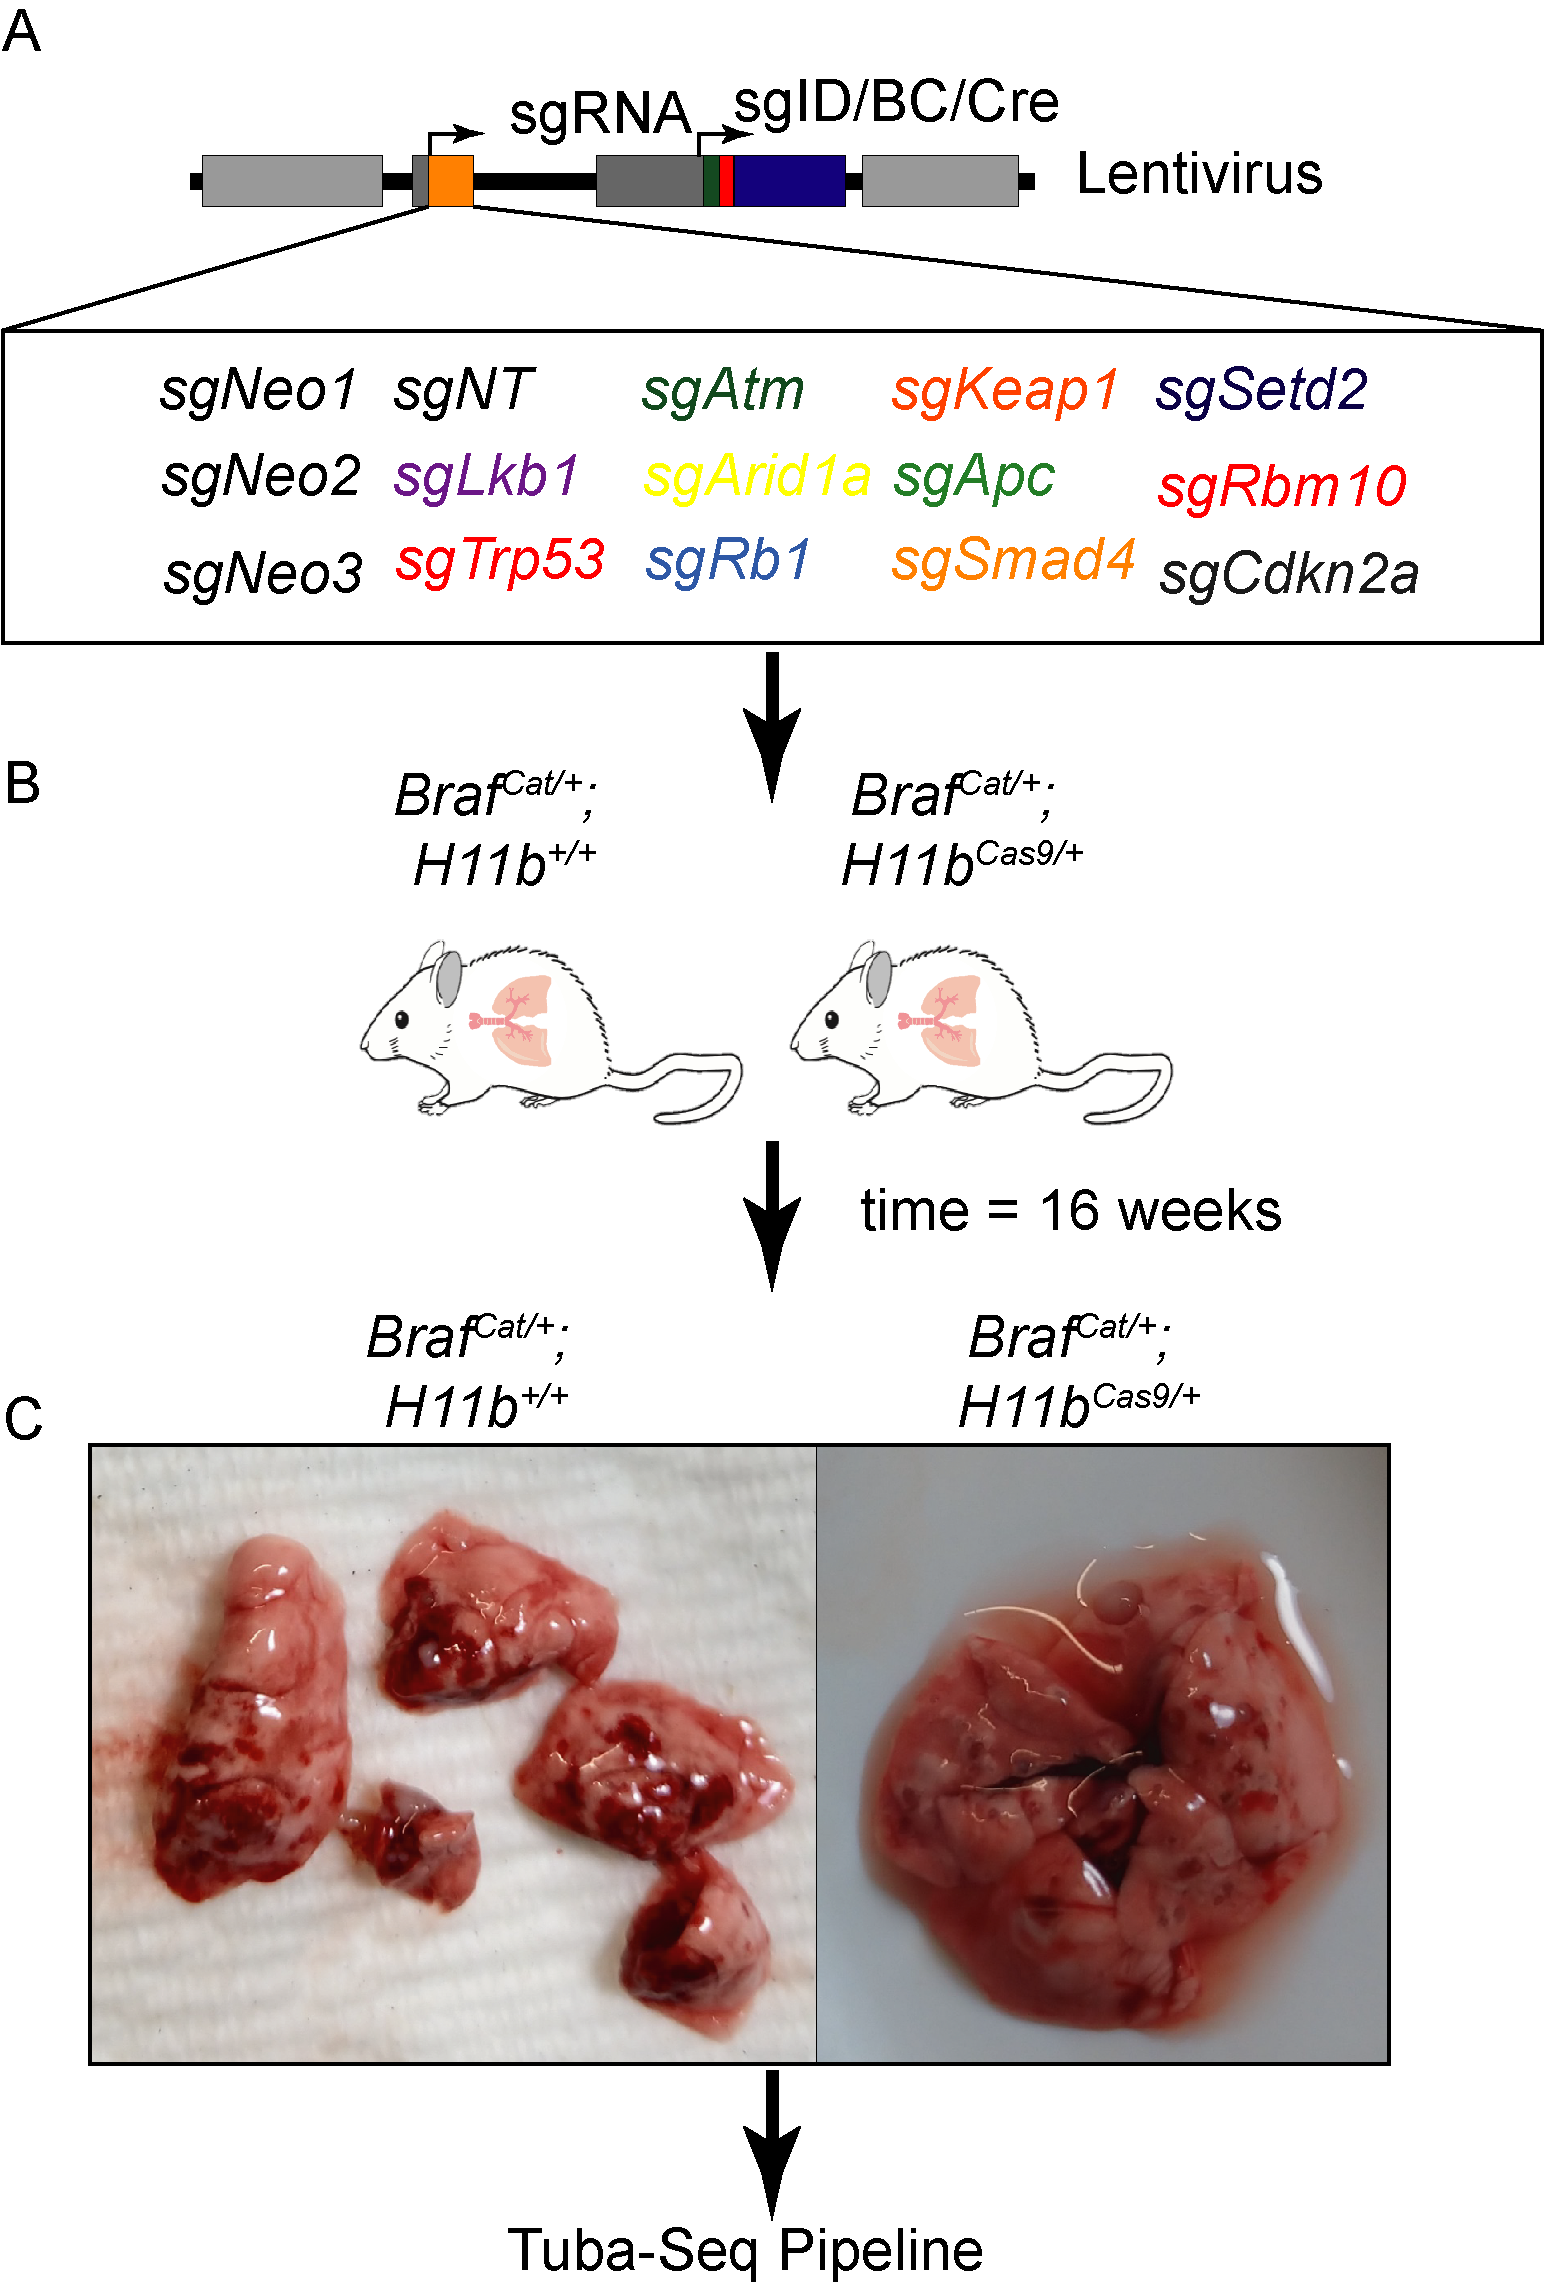
\includegraphics[width=1\textwidth,height=\textheight]{images/tuba1.png}
\caption{\textbf{This is the title of Figure} this is the text.}\label{fig:04}
}
\end{figure}

\begin{figure}
\hypertarget{fig:05}{%
\centering
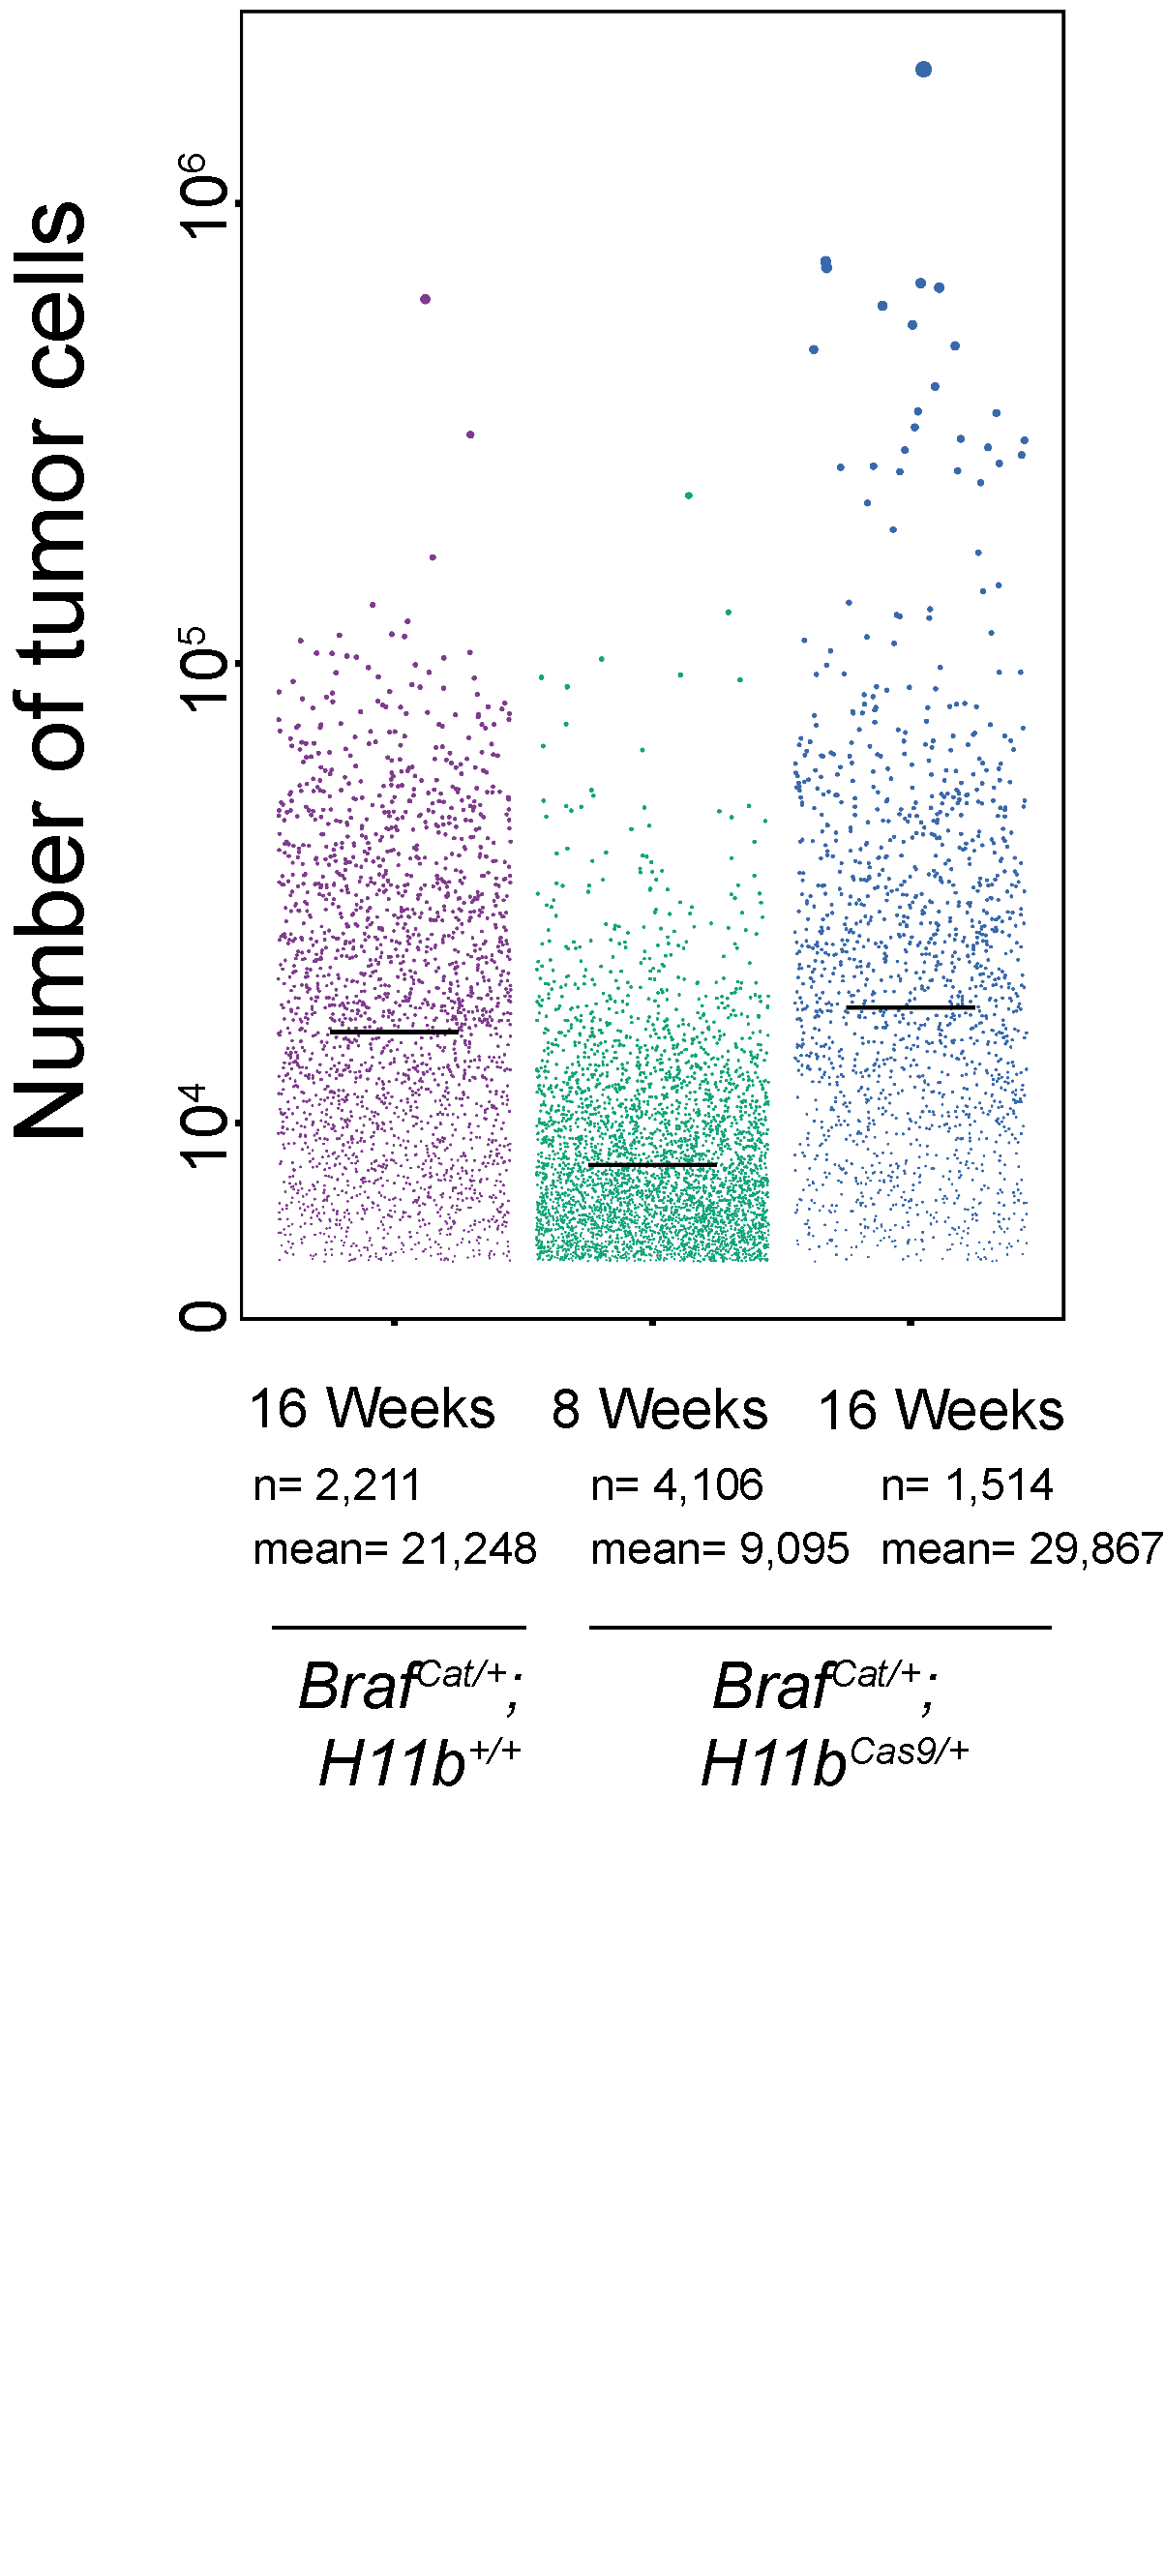
\includegraphics[width=1\textwidth,height=\textheight]{images/tuba2.png}
\caption{\textbf{This is the title of Figure} this is the text.}\label{fig:05}
}
\end{figure}

\begin{figure}
\hypertarget{fig:06}{%
\centering
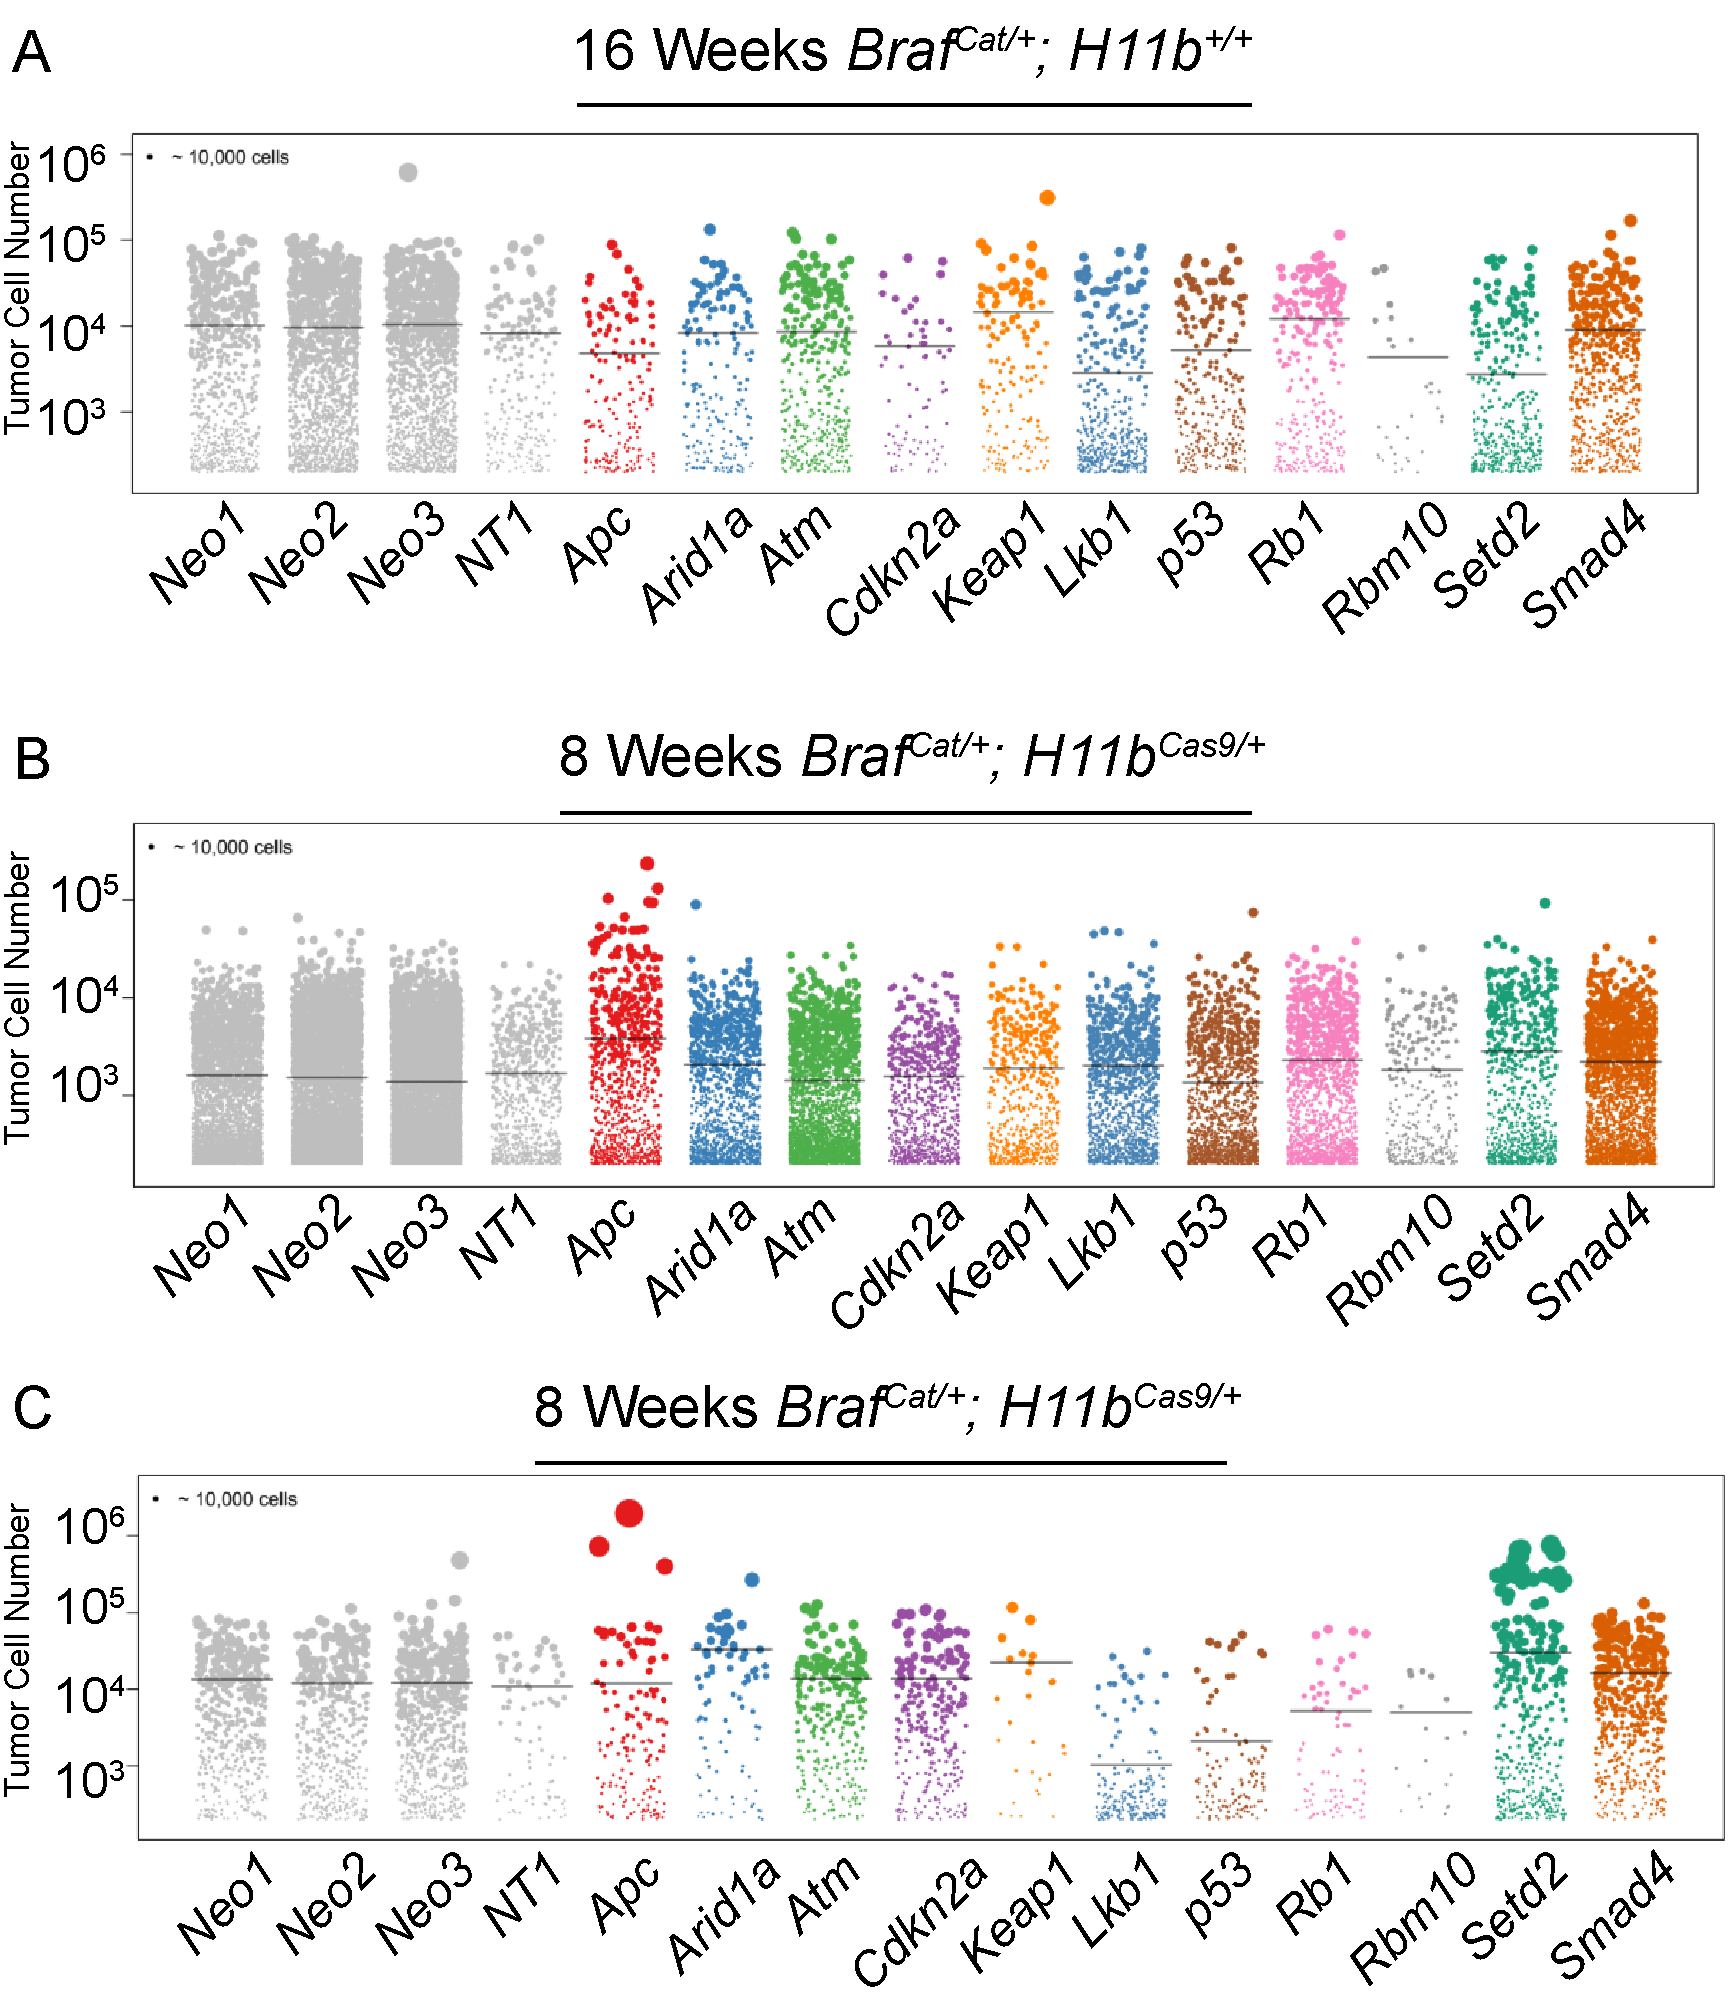
\includegraphics[width=1\textwidth,height=\textheight]{images/tuba3.png}
\caption{\textbf{This is the title of Figure} this is the text.}\label{fig:06}
}
\end{figure}

\begin{figure}
\hypertarget{fig:07}{%
\centering
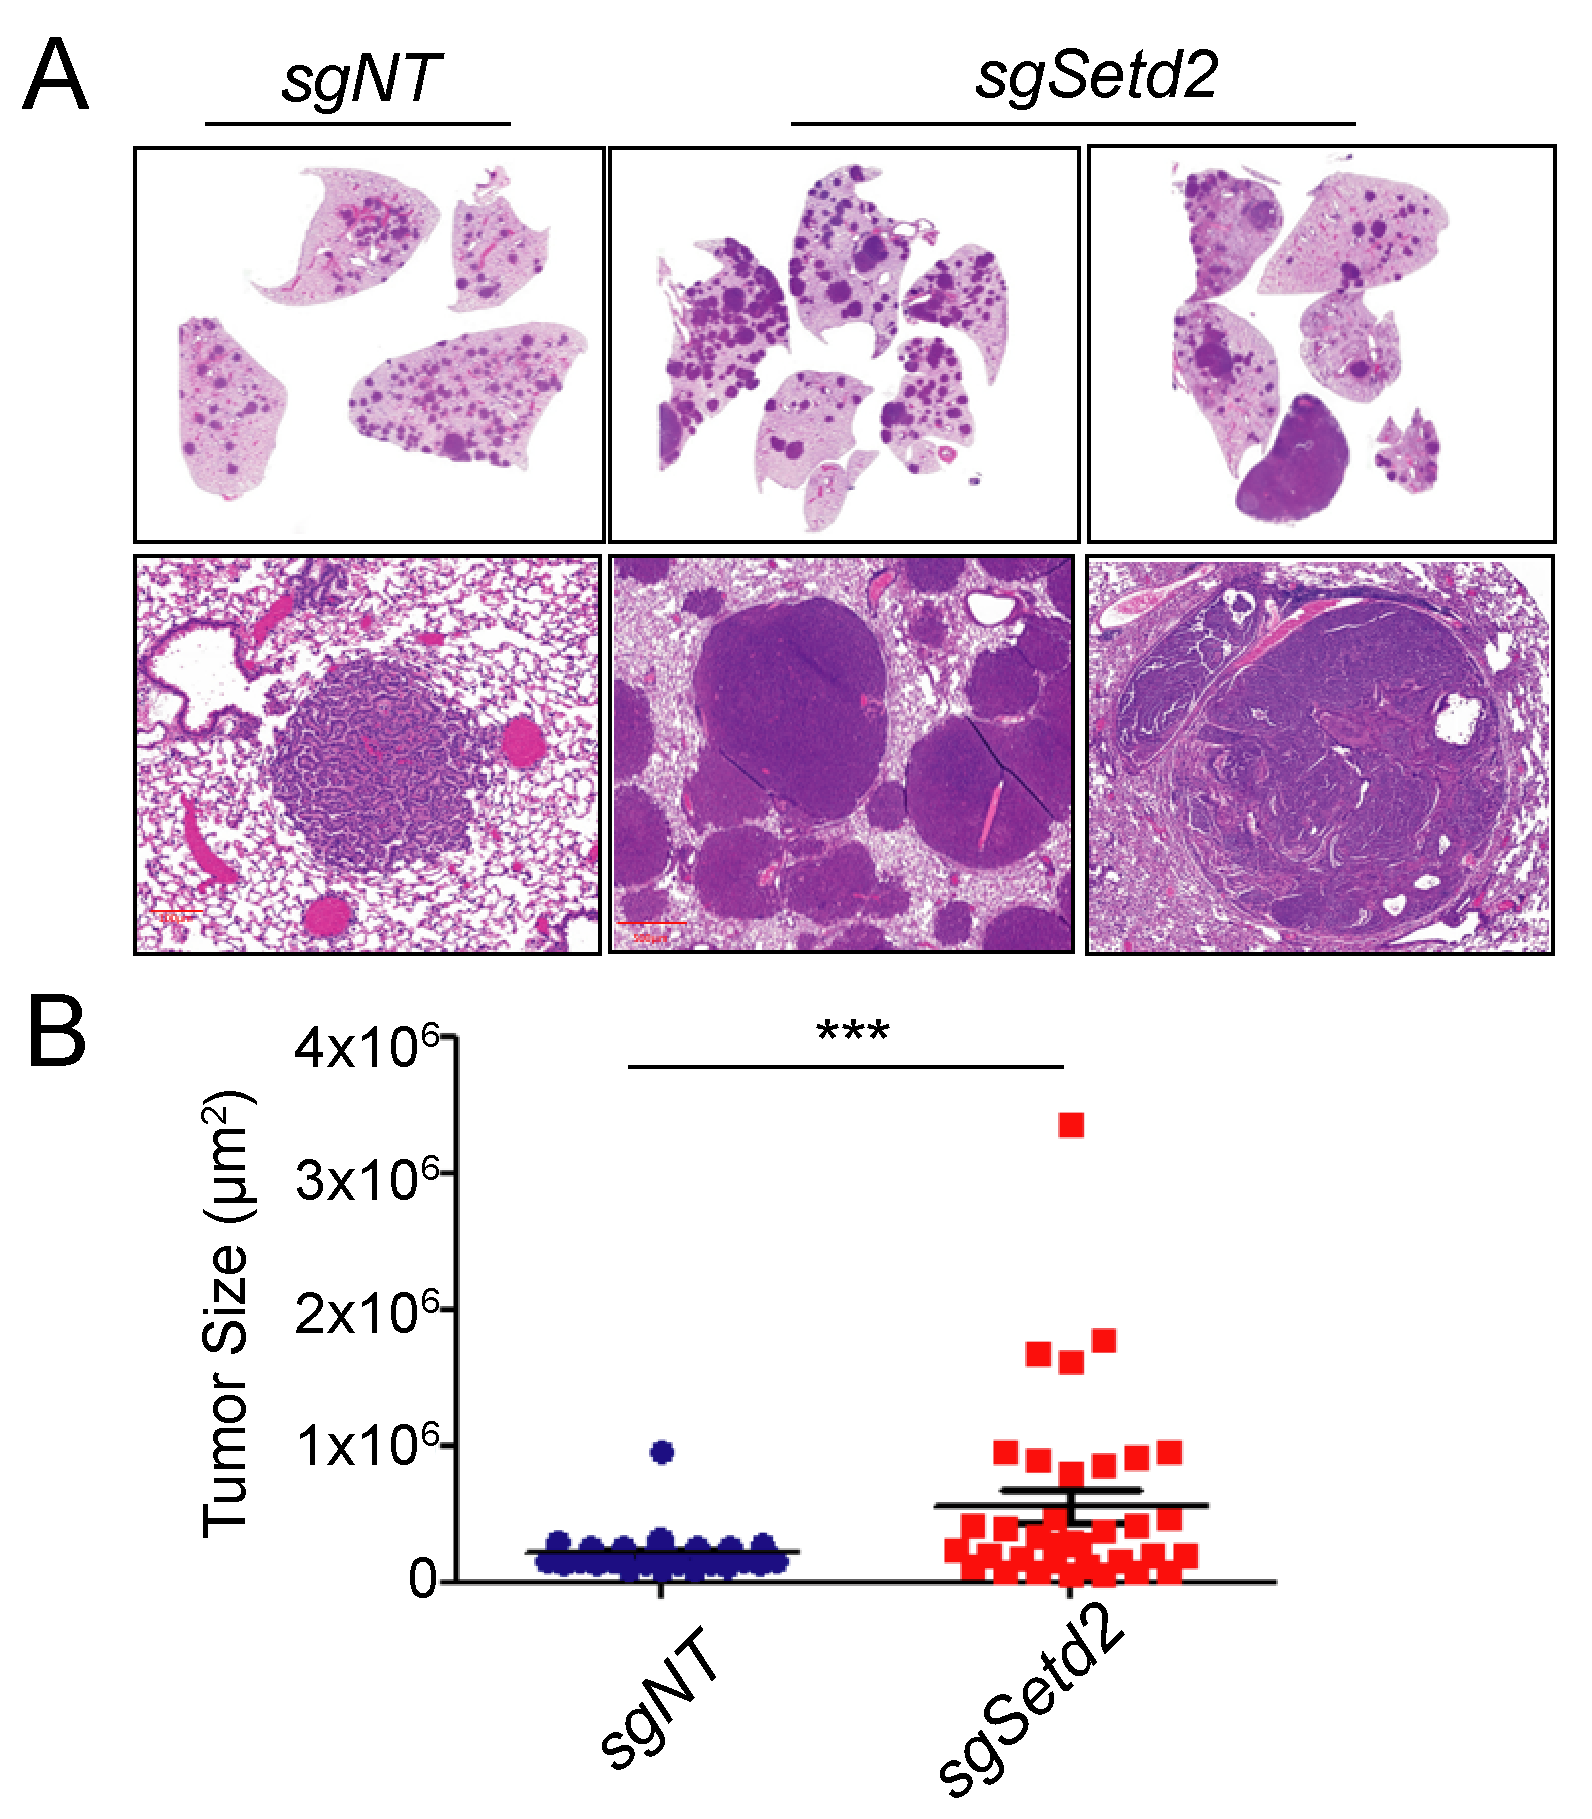
\includegraphics[width=1\textwidth,height=\textheight]{images/tuba4.png}
\caption{\textbf{This is the title of Figure} this is the text.}\label{fig:07}
}
\end{figure}

\begin{figure}
\hypertarget{fig:08}{%
\centering
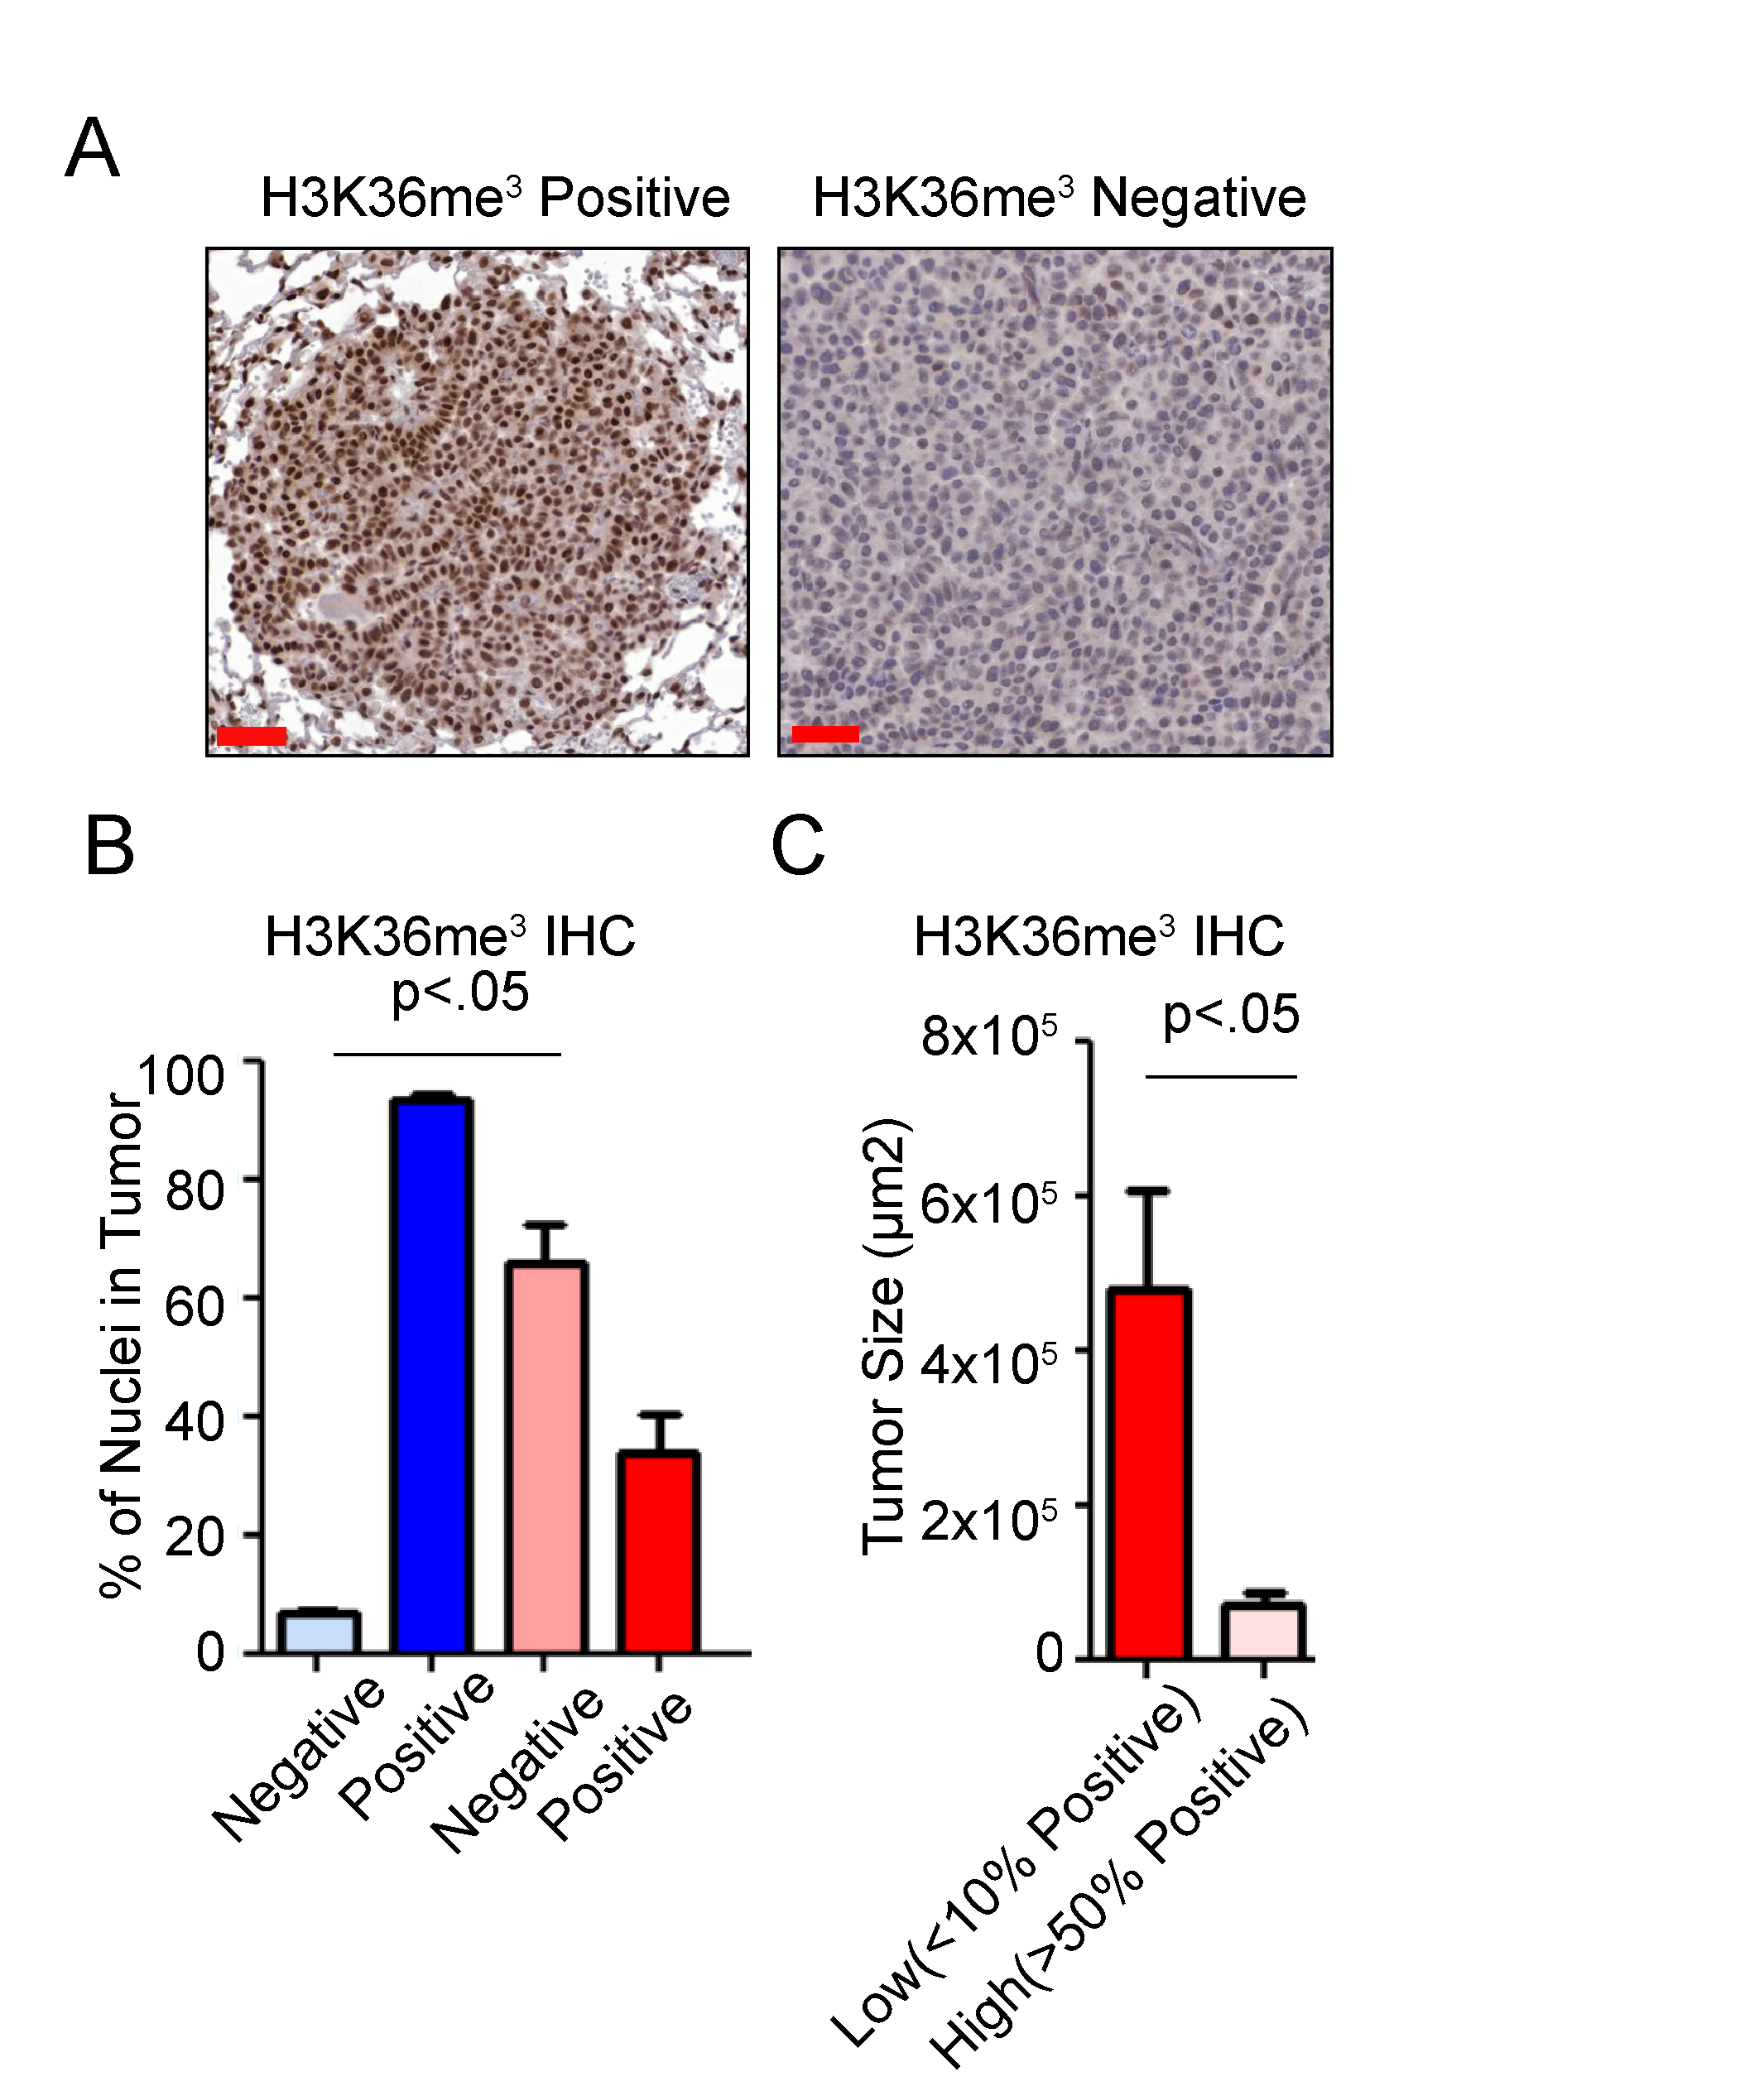
\includegraphics[width=1\textwidth,height=\textheight]{images/tuba5.png}
\caption{\textbf{This is the title of Figure} this is the text.}\label{fig:08}
}
\end{figure}

\begin{figure}
\hypertarget{fig:09}{%
\centering
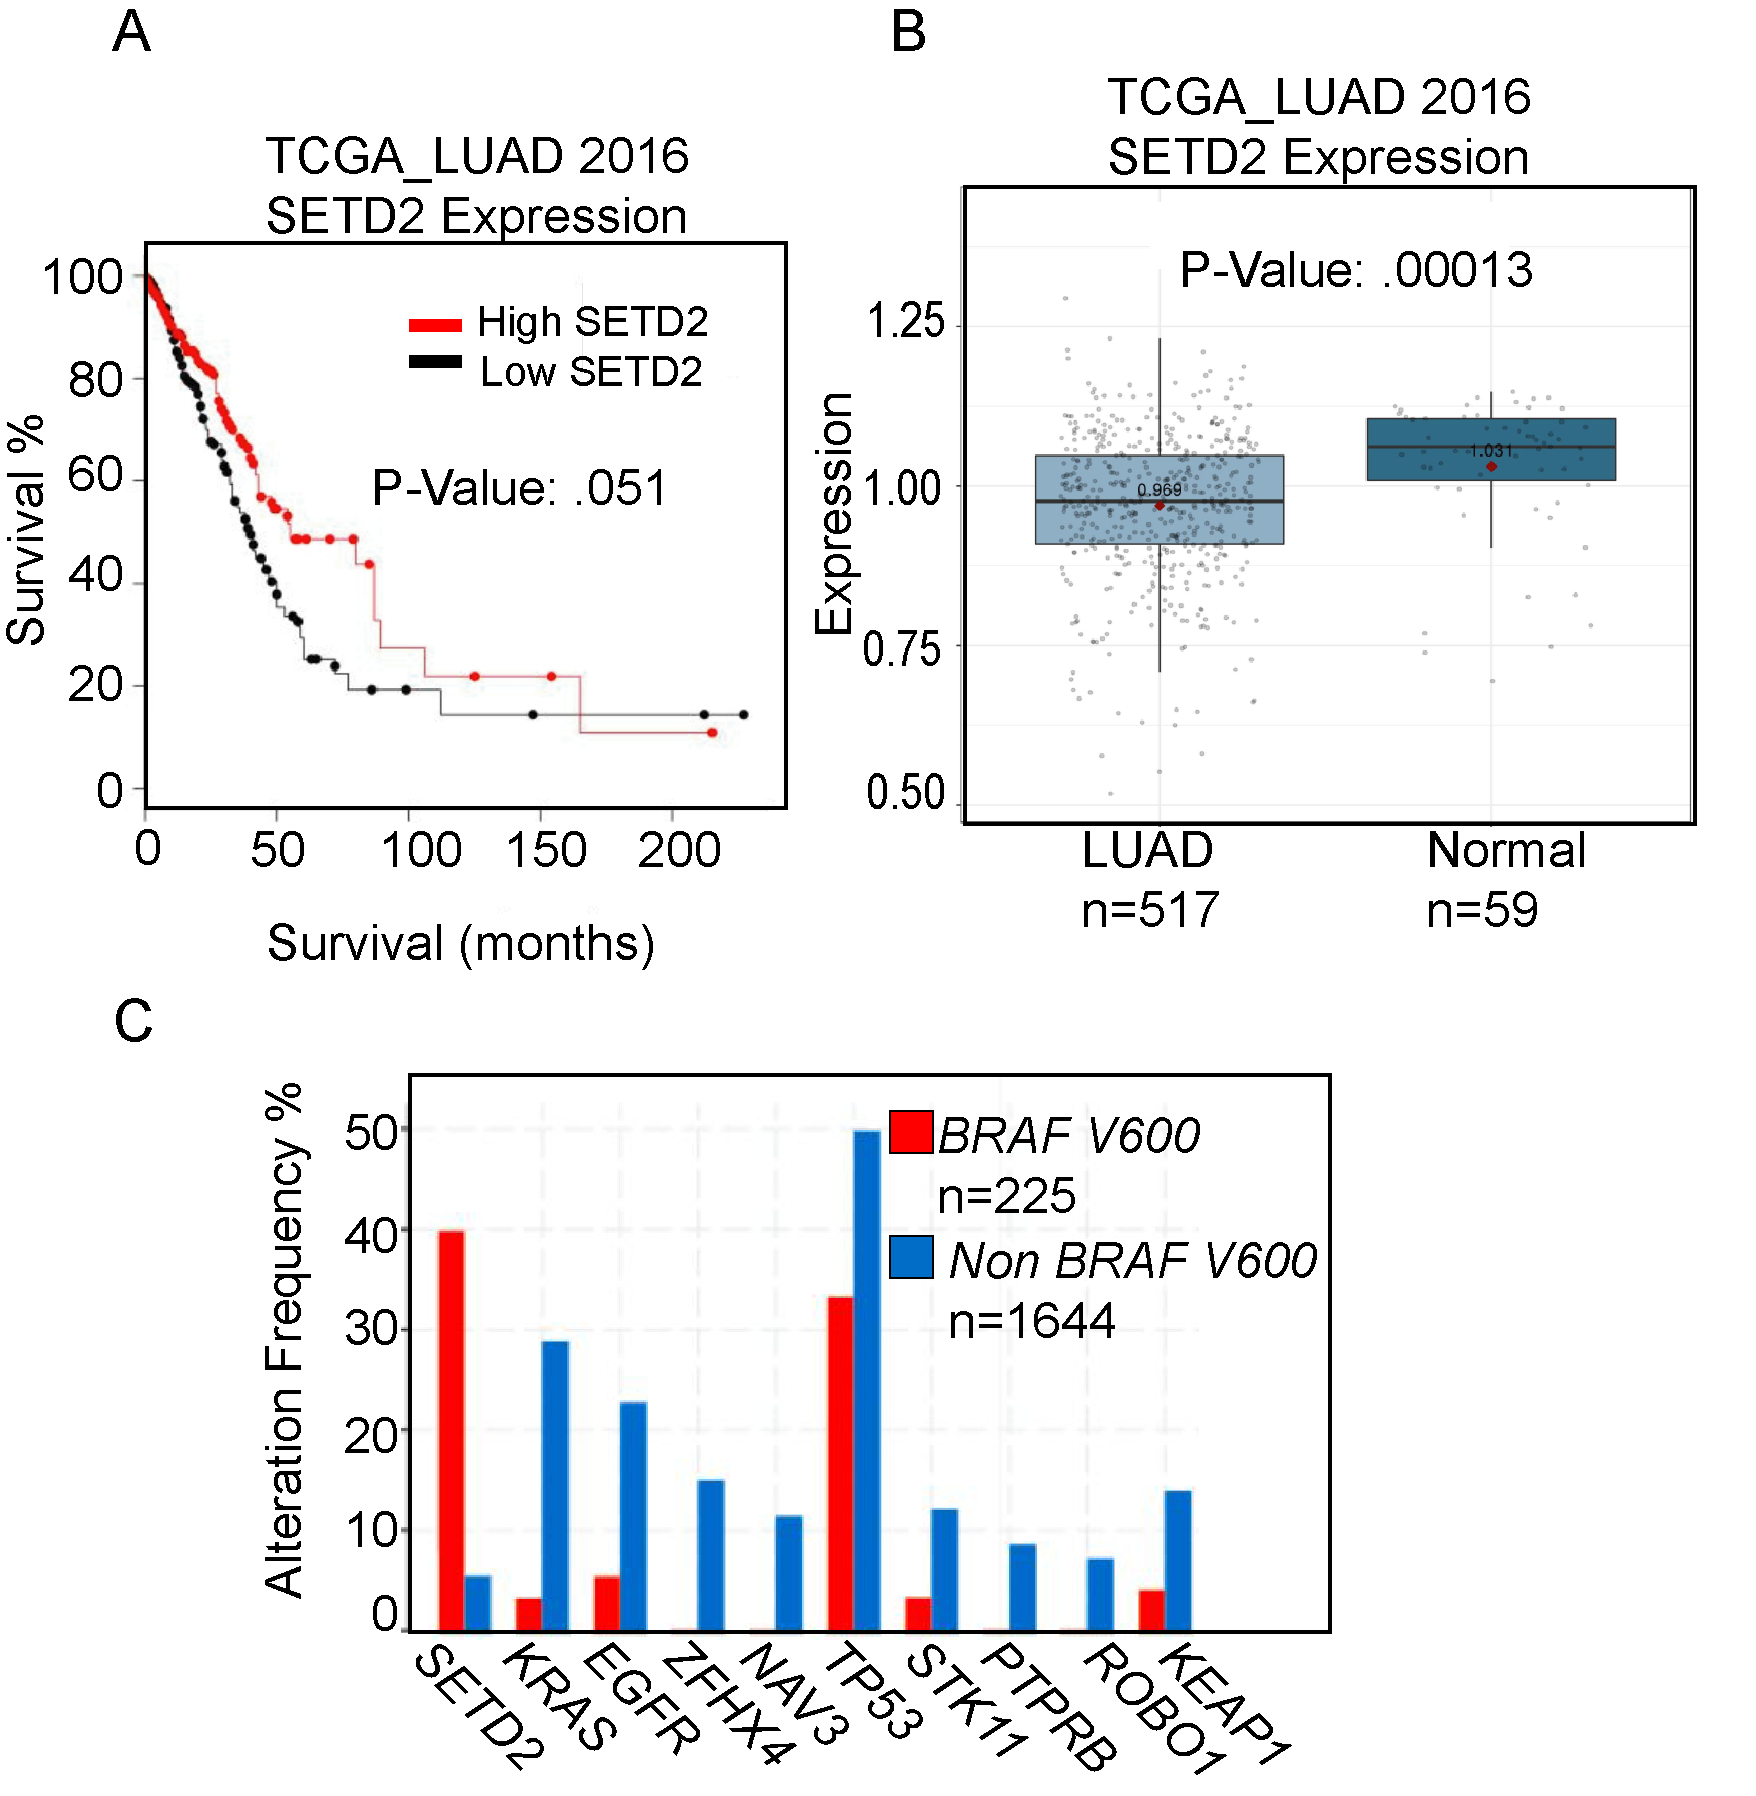
\includegraphics[width=1\textwidth,height=\textheight]{images/tuba6.png}
\caption{\textbf{This is the title of Figure} this is the text.}\label{fig:09}
}
\end{figure}

\hypertarget{chapter-three}{%
\subsection{Chapter Three}\label{chapter-three}}

\hypertarget{abstract}{%
\subsection{Abstract}\label{abstract}}

\textsuperscript{TP53} missense BRAF\textsuperscript{V600E} mutations both frequently occur in lung adenocarcinoma. While genetically engineered mouse models (GEMMs) of lung adenocarcinoma are invaluable for understanding the initiation, progression, and response to therapeutics, little is known about how different hotspot point mutations in p53 affect disease progression and therapeutic responses. To this end, we use GEMMs, tumor-derived cell lines, and human lung cancer cell lines to test how murine homologues of p53 hotspot mutants R172H and R245W compare to p53-deletion. We find that conformation mutation p53\textsuperscript{R172H} drives more aggressive lung adenocarcinomas and dedifferentiation. We also observe p53\textsuperscript{R172H} and p53\textsuperscript{R245W} accumulation in only high-grade tumors that have activated ARF expression. In vitro and in vivo studies demonstrate enhanced resistance to BRAF+MEK blockade with p53\textsuperscript{R172H} and p53\textsuperscript{R245W}, a common treatment regimen for BRAF\textsuperscript{V600E} mutant patients. Mechanistically, mutant-p53 alters the transcriptome of cancer cells and enhances entry into the cell cycle.

\hypertarget{introduction-1}{%
\subsection{Introduction}\label{introduction-1}}

Lung adenocarcinoma (LUAD) remains deadliest form of cancer since 1987 (Siegel, Miller et al.~2021). It is characterized by alterations in the MAP kinase (MAPK) pathway, including activating mutations in the oncoproteins EGFR, KRAS (G12C, G12D, G12V) or BRAF\textsuperscript{V600E} (2014; Politi \emph{et al.}, 2006; Jackson \emph{et al.}, 2001; Dankort \emph{et al.}, 2007). The recognized predominant cell of origin for LUAD, lung alveolar type-2 pneumocyte cells (AT2), are exquisitely responsive to the transformative properties of constitutive activation of the MAPK pathway (Sutherland \emph{et al.}, 2014; Sainz de Aja and Kim, 2020). Indeed, conditionally genetically engineered mouse models (GEMMs) of mutationally activated EGFR, KRAS, or BRAF form lung tumors that strongly resemble key characteristics of human LUAD. However, tumors formed in all three models (KRAS:G12D, EGFR: Deletion 19 or L858R, or BRAF:V600E) develop only into histologically low- to mid-grade cancer and are growth arrested (Jackson \emph{et al.}, 2001; Politi \emph{et al.}, 2006; Dankort \emph{et al.}, 2007). Prior research has determined that oncogene-induced tumor growth arrest occurs through activation of several tumor suppression mechanisms, most notably, p53-mediated tumor suppression (Shai \emph{et al.}, 2015).

Alterations in the \emph{TP53} tumor suppressor gene are common in all cancer types, including LUAD (Bouaoun \emph{et al.}, 2016). P53 encodes a transcription factor that responds to a variety of cell stresses, such as DNA damage and oncogene activation. In response to stress, p53 is stabilized and induces anti-proliferative and genome-mending effects through trans-activation of a diverse set of P53-target genes (Boutelle and Attardi, 2021; Vogelstein \emph{et al.}, 2000). p53 mutations observed in cancer frequently occur in the DNA binding domain where a single amino acid change results in dysfunctional DNA-binding and failed transcriptional activation (Olivier \emph{et al.}, 2010). Therefore, mutated p53 that is defunct in p53 transcriptional regulation results in failed tumor suppression and cancer outgrowth. Furthermore, defective p53 signaling will permit future genomic insults to remain unchecked thus fostering an environment primed for malignant potential. Since mutant-p53 lacks transcriptional activity through its inability to bind DNA, it is unable to induce expression of its negative regulators, ARF, MDM2 and MDMX (Perry \emph{et al.}, 1993; Wu \emph{et al.}, 1993). Lack of negative feedback results in mutant-p53 stabilization. Accumulation of mutant p53 has been reported to elicit gain-of-function p53 activity. Thus, any gain-of-function activity in mutant-p53 cannot be studied with p53-genetic deletion. Many research groups have characterized gain-of-function phenotypes of mutant-p53 in cancer. For instance, mice expressing mutant-p53 have altered disease phenotype compared to p53-null models (Olive \emph{et al.}, 2004; Lang \emph{et al.}, 2004). Specifically in lung cancer model systems, mutant-p53 has been observed to modulate SMAD3, NF\(\kappa\)B, p63, TGF\(\beta\), and others to drive various hallmarks of cancer such as invasion, chemoresistance, metabolism, and propagation of a stem cell fate (Klemke \emph{et al.}, 2021 ; Gaiddon \emph{et al.}, 2001; Adorno \emph{et al.}, 2009). Although the mechanisms that leads to these altered processes are controversial, it is thought that the main affect is through mutant-p53 binding and sequestering known p53-associated proteins. This often leads to activation of transcription factors such as NF-Y (Kim \emph{et al.}, 2021).

In BRAF\textsuperscript{V600E} GEMMs, when p53 function is abolished by \emph{Trp53} gene deletion or by \emph{Cdkn2a} deletion, lung tumors can escape growth arrest and undergo malignant transformation (Dankort \emph{et al.}, 2007; Shai \emph{et al.}, 2015). Furthermore, p53 pathway dysregulation allows a cell to sample diverse phenotypic landscapes that allow for enhanced cell fitness and tumor outgrowth (Marjanovic \emph{et al.}, 2020). However, BRAF\textsuperscript{V600E} lung tumorigenesis and progression to malignant lung adenocarcinoma has only been studied in the context of p53 genetic deletion, not p53 mutation, which are more frequently seen in human lung cancer. Specifically, p53-R172H and p53-R245W are murine homologues of common hotspots in human cancer R175H and R245W, respectively.

Here, we characterize the differential impact of p53(null), as well as p53 hotspot mutations p53\textsuperscript{R712H} (R175H in humans) and p53\textsuperscript{R245W} (R248W in humans) on BRAF\textsuperscript{V600E} lung tumorigenesis. We observed significantly differential effects of p53-R172H on BRAF\textsuperscript{V600E}-driven lung tumorigenesis that was not observed when p53 is deleted, such as enhanced tumor size and decreased survival. Our findings highlight functional differences in mutant-p53 biology, as well as the importance and the utility of clinically relevant mutant-p53 mouse models.

\hypertarget{results-1}{%
\subsection{Results}\label{results-1}}

\emph{\textbf{P53-mutant Alleles Differentially Alter BRAF (V600E) Lung Tumorigenesis}}

Expression of BRAF\textsuperscript{V600E} in the distal epithelium of the mouse lung elicits clonal tumorigenic outgrowths of alveolar type 2 (AT2) pneumocytes (Dankort et al.~2007).Prior work has shown that \emph{Trp53\textsuperscript{fl/fl}} cooperates with BRAF(V600E) to form malignant lung tumors when Cre recombinase is activated (Dankort \emph{et al.}, 2007; Shai \emph{et al.}, 2015). Therefore, we compared the tumor burden of \emph{Braf\textsuperscript{Cat/+}} mice with either p53 loss (\emph{Trp53\textsuperscript{fl/fl}}, p53\textsuperscript{R172H} (\emph{Trp53\textsuperscript{R172H/R172H}}), or p53\textsuperscript{R245W} (\emph{Trp53\textsuperscript{R245W/R245W}}) after infection with 106 pfu of adenovirus expressing surfactant protein C specific Cre (ad5-Spc-Cre) (Figure \ref{fig:11} A). As expected, mice developed lung cancer, consistent with previous findings (Figure \ref{fig:11} B-C). However, there was a striking, highly reproducible increase in the tumor size of tumors harboring \emph{Trp53\textsuperscript{R172H/R172H}} and to a lesser extent \emph{Trp53\textsuperscript{R245W/R245W}}, compared to \emph{Trp53\textsuperscript{fl/fl}} (Figure \ref{fig:11} B-D). These data led us to hypothesize that p53\textsuperscript{R172H} and p53\textsuperscript{R245W} expression alters tumor progression uniquely from p53 deletion, and these differences may be potentially evident of gain-of-function effects imparted by mutant-53. Since lung cancer patients with mutations in \emph{TP53} often start only have one mutated \emph{p53} allele unless loss of heterozygosity (LOH) occurs. Therefore, we generated mice heterozygous for both \emph{Braf\textsuperscript{CAT}} and either \emph{Trp53\textsuperscript{fl}} , \emph{Trp53\textsuperscript{R172H}}, or \emph{Trp53\^{} R245W\^{}} and observed their survival over time (Figure \ref{fig:11} E). We noted that \emph{Trp53\textsuperscript{R172H/+}} mice had diminished median overall survival compared to \emph{Trp53\textsuperscript{fl/+}} mice (183 days and 216 days), with \emph{Trp53\textsuperscript{R245W/+}} mice falling in between the two groups (median survival 212 days) (Figure \ref{fig:11} E).

We observed a distinct separation of survival between mice harboring lung tumors that are either \emph{Trp53\textsuperscript{fl/+}}, \emph{Trp53\textsuperscript{R172H/+}}, and \emph{Trp53\textsuperscript{R245W/+}}, this separation is diminished when altered p53 alleles are homozygous (Figure \ref{fig:11} F). \emph{Trp53\textsuperscript{R172H/R172H}} mice have a median survival of 120 days while \emph{Trp53\textsuperscript{fl/fl}} mice have a median survival of 136 days. Importantly, this observed difference in survival is statistically significant (Log-rank test p\textless{} 0.001) and is likely a reflection of worse diseased, characterized by enhanced tumor burden and tumor size.

\emph{\textbf{Mutant-p53 Accumulation is Associated with Dedifferentiation and p19 Induction}}

Increased malignancy in lung adenocarcinoma is often associated with altered states of tumor cell identity and dedifferentiation (van Veen \emph{et al.}, 2019; Marjanovic \emph{et al.}, 2020). Since LUADs often arise from AT2 cells, we surveyed the expression of AT2 cell identifiers, such as NKX2-1, a master regulator of AT2 transcriptional programs, and SPC, a marker of differentiated AT2 cells (Marjanovic \emph{et al.}, 2020). Quantification of over 50 tumors from \emph{Braf\textsuperscript{V600E/+}} mice with either \emph{Trp53\^{} flfl\^{}}, \emph{Trp53\textsuperscript{R172H/R172H}}, and \emph{Trp53\textsuperscript{R245W/R245W}} revealed that \emph{Trp53\textsuperscript{R172H/R1722H}} mice had significantly more tumors that stained negative for NKX2-1 and SPC (Figure \ref{fig:12} A an B). This finding strongly indicates that mutant-p53 tumors are dedifferentiated. Since HMGA2 expression is associated with LUAD dedifferentiation and worse patient prognosis, we performed IHC for HMGA2 (Cite). We noted an increase in HMGA2-positive tumors in both \emph{Trp53\textsuperscript{R172H/R172H}}, and \emph{Trp53\textsuperscript{R245W/R245W}} tumors compared to \emph{Trp53\textsuperscript{fl/fl}} (Figure \ref{fig:12} A,B). Thus, this data taken together reveals that Trp53R172H/R172H mice exhibit both a higher tumor burden and worse overall survival than \emph{Trp53\textsuperscript{fl/fl}}, but the tumors developed in these mice are more likely to exhibit malignant progression and dedifferentiation.

One striking feature of lung tumors in mice either heterozygous or homozygous for \emph{Trp53 \textsuperscript{R172H}} or \emph{Trp53\textsuperscript{R245W}} is how few tumors and tumor cells have detectable levels of mutant-p53 protein as measured by Immunohistochemistry (IHC). One critical aspect of normal p53 function is self-regulation through transcriptional activation of its negative regulator MDM2 (Wu \emph{et al.}, 1993). Thus, we predicted that homozygous p53 mutant-cells would exhibit increased mutant-p53 protein. Interestingly, in our models, we observed mutant p53 protein accumulation is restricted to malignant cells exhibited by lack of papillary architecture and nuclear atypia (Figure \ref{fig:12} C). Indeed, p53 immunostaining is correlated with increased phospho-ERK1/2 detection (Figure \ref{fig:12} D). Moreover, immunofluorescence of p53 and its positive regulator, p19/ARF, reveal cells with high p19/ARF are also high in p53 accumulation (Figure \ref{fig:12} D). This result suggests that even in homozygous mutant\_Trp53\_ mice, there is still a barrier to mutant-p53 accumulation, and our data suggests that elevated levels of p19/ARF is important for mutant-p53 accumulation, even with homozygous p53 mutations. Collectively, these data indicate that \emph{Trp53\textsuperscript{R172H}} drives more aggressive lung adenocarcinoma formation in BRAF(V600E) driven mouse models of lung cancer.

\emph{\textbf{P53\textsuperscript{R172H} and P53\textsuperscript{R245W} cell lines are refractory to BRAF/MEK inhibition}}

Given that previous research has determined that p53 mutations can confer resistance to both chemotherapies and pathway-targeted therapies (Rusch \emph{et al.}, 1995; Huang \emph{et al.}, 2011), we next questioned whether our p53 alterations would be sufficient to drive therapeutic resistance in BRAF\textsuperscript{V600E}-driven cell lines exposed to pathway-targeted therapeutics commonly administered to BRAF\textsuperscript{V600E} mutant patients, such as the combination of dabrafenib (BRAFi) plus trametinib (MEKi) (Planchard \emph{et al.}, 2016). Cell lines were derived from \emph{Braf\textsuperscript{CAT/+}} murine tumors expressing either \emph{Trp53\textsuperscript{flfl}}, \emph{Trp53\textsuperscript{R172H/R172H}}, or \emph{Trp53\textsuperscript{R245W/R245W}}) 14 weeks after infection with ad5-Spc-Cre. Cell lines expressing either \emph{Trp53\textsuperscript{R172H/R172H}} or \emph{Trp53\textsuperscript{R245W/R245W}} were completely resistant to single agent dabrafenib and resistant to the combination of dabrafenib plus trametinib (Figure \ref{fig:13} A,B). Of note, \emph{Trp53\textsuperscript{R172H/R172H}} and \emph{Trp53\textsuperscript{R245W/R245W}} cell lines express increased ERK1/2 activity, as evidenced by increased phosphorylated ERK1/2, both with and without Dabrafenib and Trametinib (Figure \ref{fig:13} E). Moreover, \emph{Trp53\textsuperscript{R172H/R172H}} mice retain a larger tumor burden after a week 4 treatment of MAPK blockade \emph{in vivo} (Figure \ref{fig:13} E). To gain relevance to human lung cancer, we infected BRAF(V600E) mutant HCC364 cells with lentivirus expressing human cancer hotspot mutant p53\textsuperscript{R175H}. p53\textsuperscript{R175H} expressing cells were more proliferative and more refractory than parental HCC364 cells (Figure \ref{fig:13} F and G).Collectively, these \emph{in vitro} and \emph{in vivo} data suggest missense mutant p53\textsuperscript{R175H} and its murine homologue p53\textsuperscript{R172H}, as well as p53\textsuperscript{R245W} can support cancer cell viability in the face of BRAF+MEK blockade that cannot be achieved by p53-null mutations.

\emph{\textbf{P53\textsuperscript{R172H} and P53\textsuperscript{R245W} alters the transcriptome of BRAF(V600E) lung tumor cell lines}}

Due to our observations that mutant p53\textsuperscript{R172H} drives more aggressive cancer phenotypes such as increased growth, dedifferentiation, and resistance to FDA-approved therapeutics, we reasoned that this would be reflected in a change in the transcriptional landscape. This is due in part, by the transcriptional trans-activation potential by mutant p53. RNA sequencing of cell lines generated from p53-mutant mouse lung tumors do reveal transcriptomic differences between both p53\textsuperscript{R172H} and p53\textsuperscript{R245W} cells compared to p53-null cell lines (Figure \ref{fig:14} 4 A). Interestingly, genes involved in cell cycle regulation, epithelial-to-mesenchymal transition (EMT), and MYC pathway are upregulated in both p53\textsuperscript{R172H} and p53\textsuperscript{R2245W} cell lines (Figure 4 \ref{fig:14} B). These results suggest that mutant-p53 is affecting transcription of genes involved in pro-growth signaling pathways.

\begin{figure}
\hypertarget{fig:11}{%
\centering
\includegraphics[width=0.75\textwidth,height=\textheight]{images/figure.svg}
\caption{\textbf{Differential BRAF\textsuperscript{V600E} lung tumorigenesis imparted by p53-Hotspot mutants.} \textbf{(A)} Genetically-engineered alleles of \emph{Braf\textsuperscript{v600E}} and \textsuperscript{Trp53} before and after Cre-Recombinase. \textbf{(B)} Tumor burden and \emph{(C)}** Tumor size of BRAF(V600E) plus Trp53-wildtype, null, or mutant alleles 14 weeks post Cre-mediated recombination. \emph{(D)} Representative H\&E images 14 weeks after Cre-recombination. \textbf{(E)} Survival of mice with Heterozygous \emph{Trp53} mutant alleles. \textbf{(F)} Survival of mice with homozygous \emph{Trp53} alleles.}\label{fig:11}
}
\end{figure}

\begin{figure}
\hypertarget{fig:12}{%
\centering
\includegraphics[width=0.75\textwidth,height=\textheight]{images/figure2_021722.svg}
\caption{\textbf{Missense mutant-p53 alters lung adenocarcinoma differentiation status and accumulation of mutant-p53 correlates with p19 ARF expression.} \textbf{(A)} Panel representative IHC sections stained with SPC,NKX2-1, p53 and HMGA2. \textbf{(B)} H-score of individual tumors. \textbf{(C)} Association between mutant-p53 R172H accumulation and increased malignancy and dedifferentiation. \textbf{(D)} serial section of P53-HI and pERK1/2-HI tumors compared to adjacent low. \textbf{(E)} Colocalization of p19/ARF and p53 in p53-mutant tumors}\label{fig:12}
}
\end{figure}

\begin{figure}
\hypertarget{fig:13}{%
\centering
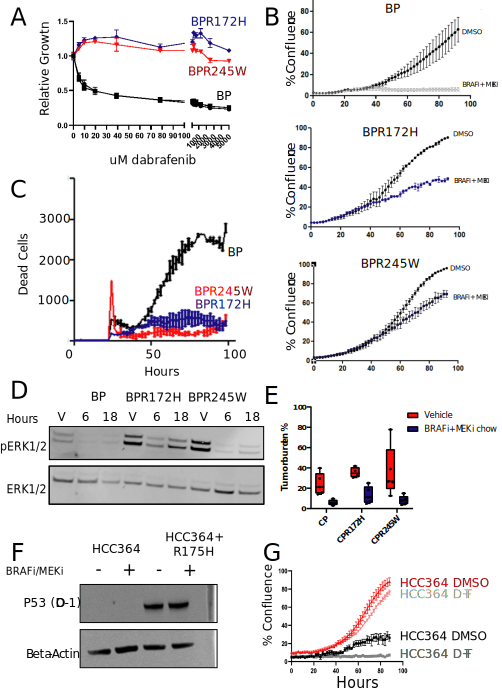
\includegraphics[width=0.75\textwidth,height=\textheight]{images/figure3_021722.svg}
\caption{\textbf{Mutant-p53 cell lines are refractory to BRAFi+MEKi.} \textbf{(A)} Response of GEMMs to BRAFi+MEKi chow after four weeks \textbf{(B)} in vitro dose response to BRAFi single agent. \textbf{(C)} in vitro timecourse with dabrafenib (1000nm) plus trametinib (100nM). \textbf{(D)} Accumulation of dead cells in dabrafenib plus trametinib measured by CytotoxRed accumulation. \textbf{(E)} Immunoblotting of phospho-ERK1/2 in response to dabrafenib plus trametinib. \textbf{(F)} Ectopic expression of p53\textsuperscript{R17H} in human HCC364 cells. \textbf{(E)} Response of p53\textsuperscript{R175H} cells to dabrafenib plus trametinib.}\label{fig:13}
}
\end{figure}

\begin{figure}
\hypertarget{fig:14}{%
\centering
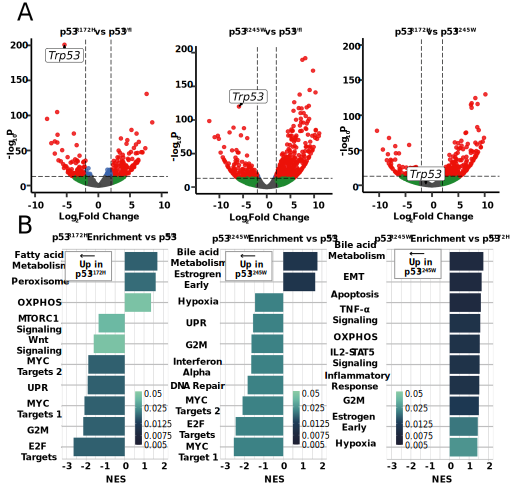
\includegraphics[width=0.75\textwidth,height=\textheight]{images/figure4_021722.svg}
\caption{\textbf{Mutant-p53 expression cells have distinct transcriptome compared to p53-null cells.} \textbf{(A)} Volcano plot of differentially-expressed genes. \textbf{(B)} Upregulated pathways using GSEA with Hallmark gene sets.}\label{fig:14}
}
\end{figure}

\hypertarget{discussion-1}{%
\subsection{Discussion}\label{discussion-1}}

While lung adenocarcinomas primarily contain missense mutations in p53, most studies using mouse models of lung adenocarcinoma utilize a p53-null (\emph{Trp53\textsuperscript{fl/fl}}) allele instead of alleles encoding hotspot missense mutations (Gao \emph{et al.}, 2013). This is most likely because prior mutant-p53 alleles were null for \emph{Trp53} prior to Cre-mediated recombination, leaving every cell in the mouse sensitive to leukemias, lymphomas and sarcomas due to being partially p53-deficient (Jackson \emph{et al.}, 2005; Wijnhoven \emph{et al.}, 2005; Olive \emph{et al.}, 2004). Our work has been made possible by newly described ``wildtype to mutant'' p53 alleles that allow for mice to be fully wildtype for p53 in all cells prior to Cre-mediated recombination(Zhang \emph{et al.}, 2018). This strategy is crucial, as it allows for temporally extended experiments not confounded by separate malignancies. Here, we utilize "wildtype to mutant"\emph{Trp53\textsuperscript{R172H}} and \emph{Trp53\textsuperscript{R245W}} alleles R245W to determine how they alter tumor progression in a BRAF(V600E) model of lung cancer. We show that p53\textsuperscript{R172H} and p53\textsuperscript{R245W} accelerates lung tumor progression and increases the rate of dedifferentiation beyond complete loss of p53 expression.

Although point mutations in the \emph{TP53} gene can poison the natural tumor suppressive mechanisms of p53 protein, not all point mutations are equivalent in executing these functions. Mutations in the DNA-binding domain are most common and most potent at ablating normal p53 function. Taking advantage of a conditional BRAF\textsuperscript{V600E} lung tumor model where BRAF\textsuperscript{V600E} expression in AT2 cells drives benign tumor formation, we show that either p53\textsuperscript{R172H} or p53\textsuperscript{R245W} can bypass growth arrest and influence tumor progression and therapeutic sensitivity beyond how p53 loss can. Specifically, P53\textsuperscript{R172H} reduces survival and sensitivity to dabrafenib plus trametinib \emph{in vivo}. Interestingly, a single allele of p53\textsuperscript{R172H} has a stronger tumor promoting phenotype than P53\textsuperscript{R245W}. These findings further support a hierarchy model of p53 missense mutations, where conformation mutants such as p53\textsuperscript{R175H} have a stronger dominant-negative effect on wildtype p53, while mice with a single \emph{trp53\textsuperscript{fl}} allele can still suppress tumorigenesis with one copy of wildtype but are prone to Loss of heterozygosity (Zhang \emph{et al.}, 2018; Muzumdar \emph{et al.}, 2016; Olive \emph{et al.}, 2004).

In BRAF-driven lung adenocarcinoma, the repressive role of wild-type p53 is initiated by oncogenic stress brought about by increasing levels of MAPK-pathway activation(Dankort \emph{et al.}, 2007) . Hyperactivation of the MAPK pathway triggers p19/ARF to block MDM2, leading to p53 accumulation(Christophorou \emph{et al.}, 2006; Feldser \emph{et al.}, 2010; Junttila \emph{et al.}, 2010). Therefore, p53 acts late in lung adenocarcinoma, in contrast to pancreatic adenocarcinoma, where p53 is triggered early likely through PDAC-specific increases in p19/ARF through either increased PI3K, STAT3, or DMP1 (Muzumdar \emph{et al.}, 2016). Our studies in BRAF(V600E) mutant lung adenocarcinomas reinforce this concept, as mutant-p53 does not accelerate growth in early tumors (supplemental figure). Furthermore, p53 is not detected until later stage tumor development and correlates with p19/ARF expression and increased phospho-ERK1/2 levels. Our studies indicate that mutant-p53 levels are associated with increased expression of p19/ARF. Therefore, any gain-of-function phenotype manifested by mutant-p53 must depend on accumulated p19/ARF. Thus, ablating the ARF tumor suppressor in human cancers with GOF \emph{TP53} mutants may paradoxically lead to tumor regression.

While most \emph{TP53} mutations observed in cancer result in an inability to bind DNA, they are often stable and preserve functional oligomerization and transcriptional transactivation domains(Garcia and Attardi, 2014). Thus, mutant-p53 can still interact with and affect the function of cellular processes. Supporting this rationale we observe altered transcriptomes with both p53\textsuperscript{R172H} and p53\^{}R245W cell lines compared to p53-null. Consistent with previous mutant-p53 GOF studies, we observed enriched genes associated with EMT and cell-cycle entry with p53\textsuperscript{R172H} and p53\textsuperscript{R245W}.

Many GOF phenotypes exhibited by mutant-p53 have centered around drug resistant mechanisms. Previous studies have shown that mutant-p53 can confer resistance to pathway targeted therapy and chemotherapies. Our studies highlight that p53\textsuperscript{R172H} and p53\textsuperscript{R245W} can confer resistance to BRAF-targeted therapy. Here, we show p53-R172H and p53-R245W cell lines are resistant to BRAF(V600E) inhibition and less sensitivity to the combination of BRAF+MEK inhibition. In pancreatic cancer models with LSL-p53-R172H expression, mutant-p53 regulates PDGFR-signaling to promote an invasive phenotype that is sensitive to Imatinib(Weissmueller \emph{et al.}, 2014). Consistent with these findings, our transcriptional analysis and immunoblotting indicate p53-R172H and p53-R245W cells express PDGF-ligands and exhibit PDGFR-pathway activation.

In summary, we have compared the tumorigenic potential of three \emph{\textsuperscript{Trp53}} alleles (\emph{Trp53\textsuperscript{fl/fl}}, \emph{Trp53\textsuperscript{R172H}}, and \emph{Trp53\textsuperscript{R245W}}) concurrently with \emph{BRAF\textsuperscript{V600E}}. \emph{Trp53\textsuperscript{R172H}} and \emph{Trp53\textsuperscript{R245W}} promoted more aggressive lung cancers exhibited by larger tumors and tumor dedifferentiation. However, only \emph{Trp53\textsuperscript{R172H}} was observed to shorten survival compared to \emph{Trp53\textsuperscript{fl/fl}}. Moreover, \emph{Trp53\textsuperscript{R172H}} and \emph{Trp53\textsuperscript{R245W}} cell lines were refractory to dabrafenib and trametinib and were more proliferative. \emph{Trp53\textsuperscript{R172H}} and \emph{Trp53\textsuperscript{R245W}} cell lines had altered transcriptomes compared to p53-null cells and were highly enriched in genes involved in cell cycle proliferation. Our work highlights the importance of studying disease-relevant \emph{TP53} alleles in pre-clinical modeling systems.

\hypertarget{chapter-four}{%
\subsection{Chapter Four}\label{chapter-four}}

\hypertarget{references}{%
\subsection{References}\label{references}}

\hypertarget{refs}{}
\begin{CSLReferences}{1}{0}
\leavevmode\vadjust pre{\hypertarget{ref-8Gf0ScB2}{}}%
(2014) \href{https://doi.org/10.1038/nature13385}{Comprehensive molecular profiling of lung adenocarcinoma.} \emph{Nature}, \textbf{511}, 543--50.

\leavevmode\vadjust pre{\hypertarget{ref-1HKPvGqty}{}}%
Adorno,M. \emph{et al.} (2009) \href{https://doi.org/10.1016/j.cell.2009.01.039}{A Mutant-p53/Smad complex opposes p63 to empower TGFbeta-induced metastasis.} \emph{Cell}, \textbf{137}, 87--98.

\leavevmode\vadjust pre{\hypertarget{ref-6j21xB75}{}}%
Arteaga,C.L. and Engelman,J.A. (2014) \href{https://doi.org/10.1016/j.ccr.2014.02.025}{ERBB receptors: from oncogene discovery to basic science to mechanism-based cancer therapeutics.} \emph{Cancer Cell}, \textbf{25}, 282--303.

\leavevmode\vadjust pre{\hypertarget{ref-ju5z9qDz}{}}%
Bouaoun,L. \emph{et al.} (2016) \href{https://doi.org/10.1002/humu.23035}{TP53 Variations in Human Cancers: New Lessons from the IARC TP53 Database and Genomics Data.} \emph{Hum Mutat}, \textbf{37}, 865--76.

\leavevmode\vadjust pre{\hypertarget{ref-GiCMgc6K}{}}%
Bougeard,G. \emph{et al.} (2008) \href{https://doi.org/10.1136/jmg.2008.057570}{Molecular basis of the Li-Fraumeni syndrome: an update from the French LFS families.} \emph{J Med Genet}, \textbf{45}, 535--8.

\leavevmode\vadjust pre{\hypertarget{ref-KlPsMirp}{}}%
Boutelle,A.M. and Attardi,L.D. (2021) \href{https://doi.org/10.1016/j.tcb.2020.12.011}{p53 and Tumor Suppression: It Takes a Network.} \emph{Trends Cell Biol}, \textbf{31}, 298--310.

\leavevmode\vadjust pre{\hypertarget{ref-G5wVcRrJ}{}}%
Christophorou,M.A. \emph{et al.} (2006) \href{https://doi.org/10.1038/nature05077}{The pathological response to DNA damage does not contribute to p53-mediated tumour suppression.} \emph{Nature}, \textbf{443}, 214--7.

\leavevmode\vadjust pre{\hypertarget{ref-JVkWOch7}{}}%
Cooper,W.A. \emph{et al.} (2013) \href{https://doi.org/10.3978/j.issn.2072-1439.2013.08.03}{Molecular biology of lung cancer.} \emph{J Thorac Dis}, \textbf{5 Suppl 5}, S479--90.

\leavevmode\vadjust pre{\hypertarget{ref-dTvhNsG9}{}}%
Dankort,D. \emph{et al.} (2007) \href{https://doi.org/10.1101/gad.1516407}{A new mouse model to explore the initiation, progression, and therapy of BRAFV600E-induced lung tumors.} \emph{Genes Dev}, \textbf{21}, 379--84.

\leavevmode\vadjust pre{\hypertarget{ref-1F86sLj5s}{}}%
de Groot,P. and Munden,R.F. (2012) \href{https://doi.org/10.1016/j.rcl.2012.06.006}{Lung cancer epidemiology, risk factors, and prevention.} \emph{Radiol Clin North Am}, \textbf{50}, 863--76.

\leavevmode\vadjust pre{\hypertarget{ref-iZbc8sIr}{}}%
Duggan,M.A. \emph{et al.} (2016) \href{https://doi.org/10.1097/pas.0000000000000749}{The Surveillance, Epidemiology, and End Results (SEER) Program and Pathology: Toward Strengthening the Critical Relationship.} \emph{Am J Surg Pathol}, \textbf{40}, e94--e102.

\leavevmode\vadjust pre{\hypertarget{ref-CMVwSV1C}{}}%
Feldser,D.M. \emph{et al.} (2010) \href{https://doi.org/10.1038/nature09535}{Stage-specific sensitivity to p53 restoration during lung cancer progression.} \emph{Nature}, \textbf{468}, 572--5.

\leavevmode\vadjust pre{\hypertarget{ref-oVtv8JOR}{}}%
Ferone,G. \emph{et al.} (2020) \href{https://doi.org/10.1101/gad.338228.120}{Cells of origin of lung cancers: lessons from mouse studies.} \emph{Genes Dev}, \textbf{34}, 1017--1032.

\leavevmode\vadjust pre{\hypertarget{ref-Vbw51s50}{}}%
Gaiddon,C. \emph{et al.} (2001) \href{https://doi.org/10.1128/mcb.21.5.1874-1887.2001}{A subset of tumor-derived mutant forms of p53 down-regulate p63 and p73 through a direct interaction with the p53 core domain.} \emph{Mol Cell Biol}, \textbf{21}, 1874--87.

\leavevmode\vadjust pre{\hypertarget{ref-gI9Yeagx}{}}%
Gao,J. \emph{et al.} (2013) \href{https://doi.org/10.1126/scisignal.2004088}{Integrative analysis of complex cancer genomics and clinical profiles using the cBioPortal.} \emph{Sci Signal}, \textbf{6}, pl1.

\leavevmode\vadjust pre{\hypertarget{ref-ztWGsqcf}{}}%
Garcia,P.B. and Attardi,L.D. (2014) \href{https://doi.org/10.1016/j.semcdb.2013.12.014}{Illuminating p53 function in cancer with genetically engineered mouse models.} \emph{Semin Cell Dev Biol}, \textbf{27}, 74--85.

\leavevmode\vadjust pre{\hypertarget{ref-hRW7rjfZ}{}}%
Ghimessy,A. \emph{et al.} (2020) \href{https://doi.org/10.1007/s10555-020-09903-9}{Current therapy of KRAS-mutant lung cancer.} \emph{Cancer Metastasis Rev}, \textbf{39}, 1159--1177.

\leavevmode\vadjust pre{\hypertarget{ref-19duX0kT0}{}}%
Herbst,R.S. \emph{et al.} (2008) \href{https://doi.org/10.1056/nejmra0802714}{Lung cancer.} \emph{N Engl J Med}, \textbf{359}, 1367--80.

\leavevmode\vadjust pre{\hypertarget{ref-17uu2v5lM}{}}%
Huang,S. \emph{et al.} (2011) \href{https://doi.org/10.1158/0008-5472.can-11-0128}{p53 modulates acquired resistance to EGFR inhibitors and radiation.} \emph{Cancer Res}, \textbf{71}, 7071--9.

\leavevmode\vadjust pre{\hypertarget{ref-cD4M6ONJ}{}}%
Jackson,E.L. \emph{et al.} (2001) \href{https://doi.org/10.1101/gad.943001}{Analysis of lung tumor initiation and progression using conditional expression of oncogenic K-ras.} \emph{Genes Dev}, \textbf{15}, 3243--8.

\leavevmode\vadjust pre{\hypertarget{ref-KKkLA3TK}{}}%
Jackson,E.L. \emph{et al.} (2005) \href{https://doi.org/10.1158/0008-5472.can-05-2193}{The differential effects of mutant p53 alleles on advanced murine lung cancer.} \emph{Cancer Res}, \textbf{65}, 10280--8.

\leavevmode\vadjust pre{\hypertarget{ref-okfbKJaD}{}}%
Junttila,M.R. \emph{et al.} (2010) \href{https://doi.org/10.1038/nature09526}{Selective activation of p53-mediated tumour suppression in high-grade tumours.} \emph{Nature}, \textbf{468}, 567--71.

\leavevmode\vadjust pre{\hypertarget{ref-o8jKDrsB}{}}%
Kim,M.P. \emph{et al.} (2021) \href{https://doi.org/10.1158/2159-8290.cd-20-1228}{Oncogenic }. \emph{Cancer Discov}, \textbf{11}, 2094--2111.

\leavevmode\vadjust pre{\hypertarget{ref-B0ClcVtn}{}}%
Klemke,L. \emph{et al.} (2021) \href{https://doi.org/10.3389/fonc.2021.642603}{The Gain-of-Function p53 R248W Mutant Promotes Migration by STAT3 Deregulation in Human Pancreatic Cancer Cells.} \emph{Front Oncol}, \textbf{11}, 642603.

\leavevmode\vadjust pre{\hypertarget{ref-V4ONQpBd}{}}%
Lang,G.A. \emph{et al.} (2004) \href{https://doi.org/10.1016/j.cell.2004.11.006}{Gain of function of a p53 hot spot mutation in a mouse model of Li-Fraumeni syndrome.} \emph{Cell}, \textbf{119}, 861--72.

\leavevmode\vadjust pre{\hypertarget{ref-13QSbJkMk}{}}%
Levine,A.J. (2020) \href{https://doi.org/10.1038/s41568-020-0262-1}{p53: 800 million years of evolution and 40 years of discovery.} \emph{Nat Rev Cancer}, \textbf{20}, 471--480.

\leavevmode\vadjust pre{\hypertarget{ref-ku3fwB6c}{}}%
Malhotra,J. \emph{et al.} (2016) \href{https://doi.org/10.1183/13993003.00359-2016}{Risk factors for lung cancer worldwide.} \emph{Eur Respir J}, \textbf{48}, 889--902.

\leavevmode\vadjust pre{\hypertarget{ref-pjuOgKHJ}{}}%
Marjanovic,N.D. \emph{et al.} (2020) \href{https://doi.org/10.1016/j.ccell.2020.06.012}{Emergence of a High-Plasticity Cell State during Lung Cancer Evolution.} \emph{Cancer Cell}, \textbf{38}, 229--246.e13.

\leavevmode\vadjust pre{\hypertarget{ref-7H88gN81}{}}%
Mollaoglu,G. \emph{et al.} (2018) \href{https://doi.org/10.1016/j.immuni.2018.09.020}{The Lineage-Defining Transcription Factors SOX2 and NKX2-1 Determine Lung Cancer Cell Fate and Shape the Tumor Immune Microenvironment.} \emph{Immunity}, \textbf{49}, 764--779.e9.

\leavevmode\vadjust pre{\hypertarget{ref-cWKMNUBI}{}}%
Mukhopadhyay,A. and Oliver,T.G. (2014) \href{https://doi.org/10.4161/23723548.2014.969651}{Mighty mouse breakthroughs: a Sox2-driven model for squamous cell lung cancer.} \emph{Mol Cell Oncol}, \textbf{2}, e969651.

\leavevmode\vadjust pre{\hypertarget{ref-7Yb2p7xx}{}}%
Muzumdar,M.D. \emph{et al.} (2016) \href{https://doi.org/10.1038/ncomms12685}{Clonal dynamics following p53 loss of heterozygosity in Kras-driven cancers.} \emph{Nat Commun}, \textbf{7}, 12685.

\leavevmode\vadjust pre{\hypertarget{ref-Co9gQ0V6}{}}%
Nikitin,A.Y. \emph{et al.} (2004) \href{https://doi.org/10.1158/0008-5472.can-03-3376}{Classification of proliferative pulmonary lesions of the mouse: recommendations of the mouse models of human cancers consortium.} \emph{Cancer Res}, \textbf{64}, 2307--16.

\leavevmode\vadjust pre{\hypertarget{ref-MLY9vR0E}{}}%
Olive,K.P. \emph{et al.} (2004) \href{https://doi.org/10.1016/j.cell.2004.11.004}{Mutant p53 gain of function in two mouse models of Li-Fraumeni syndrome.} \emph{Cell}, \textbf{119}, 847--60.

\leavevmode\vadjust pre{\hypertarget{ref-1Aj9gKIb1}{}}%
Olivier,M. \emph{et al.} (2010) \href{https://doi.org/10.1101/cshperspect.a001008}{TP53 mutations in human cancers: origins, consequences, and clinical use.} \emph{Cold Spring Harb Perspect Biol}, \textbf{2}, a001008.

\leavevmode\vadjust pre{\hypertarget{ref-E3yjcNvW}{}}%
Perry,M.E. \emph{et al.} (1993) \href{https://doi.org/10.1073/pnas.90.24.11623}{The mdm-2 gene is induced in response to UV light in a p53-dependent manner.} \emph{Proc Natl Acad Sci U S A}, \textbf{90}, 11623--7.

\leavevmode\vadjust pre{\hypertarget{ref-BpRBkUVl}{}}%
Planchard,D. \emph{et al.} (2016) \href{https://doi.org/10.1016/s1470-2045(16)30146-2}{Dabrafenib plus trametinib in patients with previously treated BRAF(V600E)-mutant metastatic non-small cell lung cancer: an open-label, multicentre phase 2 trial.} \emph{Lancet Oncol}, \textbf{17}, 984--993.

\leavevmode\vadjust pre{\hypertarget{ref-kQzAqqtP}{}}%
Politi,K. \emph{et al.} (2006) \href{https://doi.org/10.1101/gad.1417406}{Lung adenocarcinomas induced in mice by mutant EGF receptors found in human lung cancers respond to a tyrosine kinase inhibitor or to down-regulation of the receptors.} \emph{Genes Dev}, \textbf{20}, 1496--510.

\leavevmode\vadjust pre{\hypertarget{ref-PX0Ki15S}{}}%
Rusch,V. \emph{et al.} (1995) \href{https://www.ncbi.nlm.nih.gov/pubmed/7585548}{Aberrant p53 expression predicts clinical resistance to cisplatin-based chemotherapy in locally advanced non-small cell lung cancer.} \emph{Cancer Res}, \textbf{55}, 5038--42.

\leavevmode\vadjust pre{\hypertarget{ref-UfKKrJ6l}{}}%
Sainz de Aja,J. and Kim,C.F. (2020) \href{https://doi.org/10.1016/j.cell.2019.12.020}{May the (Mechanical) Force Be with AT2.} \emph{Cell}, \textbf{180}, 20--22.

\leavevmode\vadjust pre{\hypertarget{ref-Ntv29NRu}{}}%
Shai,A. \emph{et al.} (2015) \href{https://doi.org/10.1158/0008-5472.can-14-3701}{TP53 Silencing Bypasses Growth Arrest of BRAFV600E-Induced Lung Tumor Cells in a Two-Switch Model of Lung Tumorigenesis.} \emph{Cancer Res}, \textbf{75}, 3167--80.

\leavevmode\vadjust pre{\hypertarget{ref-gY2NonCA}{}}%
Siegel,R.L. \emph{et al.} (2021) \href{https://doi.org/10.3322/caac.21654}{Cancer Statistics, 2021}. \emph{CA A Cancer J. Clin.}, \textbf{71}, 7--33.

\leavevmode\vadjust pre{\hypertarget{ref-dAZ32h3a}{}}%
Sutherland,K.D. \emph{et al.} (2014) \href{https://doi.org/10.1073/pnas.1319963111}{Multiple cells-of-origin of mutant K-Ras-induced mouse lung adenocarcinoma.} \emph{Proc Natl Acad Sci U S A}, \textbf{111}, 4952--7.

\leavevmode\vadjust pre{\hypertarget{ref-1GkFEmggg}{}}%
van Veen,J.E. \emph{et al.} (2019) \href{https://doi.org/10.7554/elife.43668}{Mutationally-activated PI3'-kinase-α promotes de-differentiation of lung tumors initiated by the BRAF}. \emph{Elife}, \textbf{8}.

\leavevmode\vadjust pre{\hypertarget{ref-14fESvHZW}{}}%
Vogelstein,B. \emph{et al.} (2000) \href{https://doi.org/10.1038/35042675}{Surfing the p53 network.} \emph{Nature}, \textbf{408}, 307--10.

\leavevmode\vadjust pre{\hypertarget{ref-11g54rA8N}{}}%
Warren,G.W. and Cummings,K.M. (2013) \href{https://doi.org/10.14694/edbook_am.2013.33.359}{Tobacco and lung cancer: risks, trends, and outcomes in patients with cancer.} \emph{Am Soc Clin Oncol Educ Book}, 359--64.

\leavevmode\vadjust pre{\hypertarget{ref-jHVcJWec}{}}%
Weissmueller,S. \emph{et al.} (2014) \href{https://doi.org/10.1016/j.cell.2014.01.066}{Mutant p53 drives pancreatic cancer metastasis through cell-autonomous PDGF receptor β signaling.} \emph{Cell}, \textbf{157}, 382--394.

\leavevmode\vadjust pre{\hypertarget{ref-CVOIe1Dg}{}}%
Wijnhoven,S.W.P. \emph{et al.} (2005) \href{https://doi.org/10.1158/0008-5472.can-05-1650}{Mice expressing a mammary gland-specific R270H mutation in the p53 tumor suppressor gene mimic human breast cancer development.} \emph{Cancer Res}, \textbf{65}, 8166--73.

\leavevmode\vadjust pre{\hypertarget{ref-Mb1Q4pdk}{}}%
Wu,X. \emph{et al.} (1993) \href{https://doi.org/10.1101/gad.7.7a.1126}{The p53-mdm-2 autoregulatory feedback loop.} \emph{Genes Dev}, \textbf{7}, 1126--32.

\leavevmode\vadjust pre{\hypertarget{ref-kitgYOkt}{}}%
Zhang,Y. \emph{et al.} (2018) \href{https://doi.org/10.1038/s41467-018-06146-9}{Somatic Trp53 mutations differentially drive breast cancer and evolution of metastases.} \emph{Nat Commun}, \textbf{9}, 3953.

\end{CSLReferences}
